\chapter{Testing}
\label{chap7}
Testing is important to verify how the implemented algorithms and schemes work. It is
important to know how the algorithms react to the sensor data. 
In this chapter the test setup are described. How the tests are carried out, 
some of the results and some immediate results. 


\section{Test Environment}
The test environment is two connected pipe segments. A Y-junction and an R-bend. This
pipe segments are connected, according to Figure \ref{chap7:fig-environment}.
\begin{figure}[htbp]
    \centering
    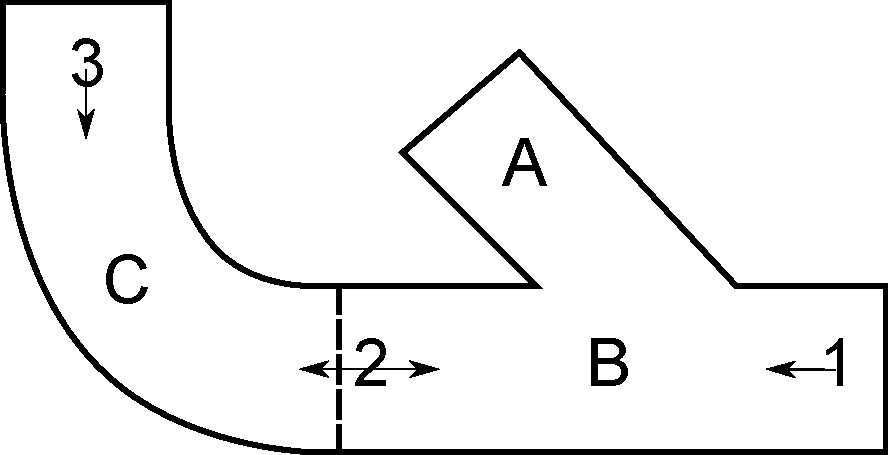
\includegraphics[width=0.6\textwidth]{pics/test-environment}
    \caption{The test environment}
    \label{chap7:fig-environment}
\end{figure}
There are five points of interest in this environment. 
The numbers \emph{1-3} are the places where the sensors will be put and record snapshots of the pipe. 
The letters \emph{B} and \emph{C} are places where irregularities and anomalies in the pipes are placed. 

The idea behind the tests is to see how the sensors and the system reacts to different
kind of anomalies, and how this impacts on the ability to detect what kind of node the
robot is approaching. 


\section{Test Cases}
To test the performance and robustness of the developed algorithms three cases are used,
ideal situation, situation with obstacles with regular surface, and obstacles where the
surface are irregular. These cases are carried out for all the 3 different places described
in the previous section.


\subsection{Control/Ideal Case}
Here the sensors are placed at the different locations and the outputs are recorded. This
is for reference and what the data will look like in the ideal case. This should
consider perfect readings and all further readings will be measured up to this.

\subsection{Long Pipe Test}
Since the implemented algorithms are best for long pipes, a test case including a
$1$ meter long pipe is included for reference. This pipe substitutes the L-bend in
shown in Figure \ref{chap7:fig-environment}. This is to test how the cylinder fit
performs. 


\subsection{Irregular surfaced anomalies}
The algorithm implemented relies greatly on regularity in the environment. The structure
of the surroundings is known to great extent and all irregularities and differences from
this are considered strange and are marked as anomalies. 

The tests are carried out with a curled-up paper which is placed at the three different
locations, marked in Figure \ref{chap7:fig-environment}. The paper is seen at position B
in the left image in Figure \ref{chap7:fig-pics-of-obstacles}.
\begin{figure}[htbp]
    \centering
    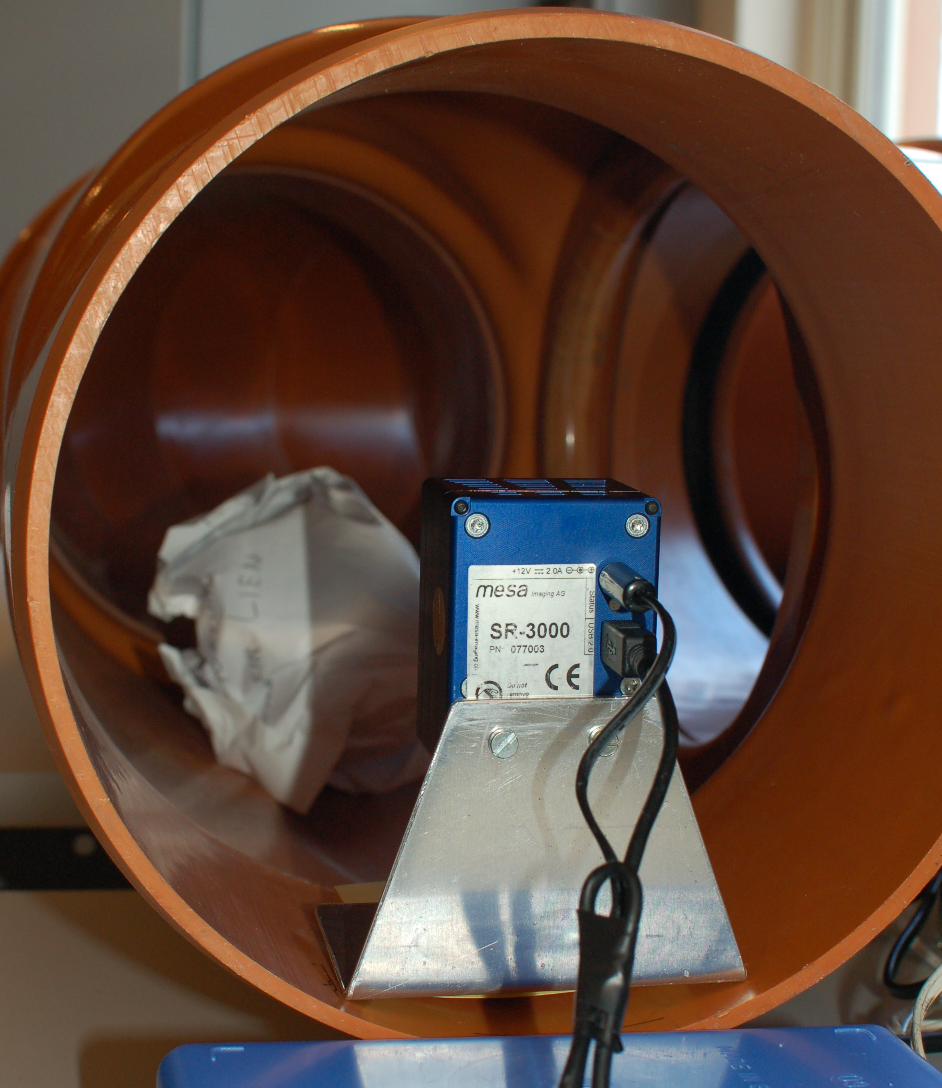
\includegraphics[width=0.47\textwidth]{pics/irregularSR}
    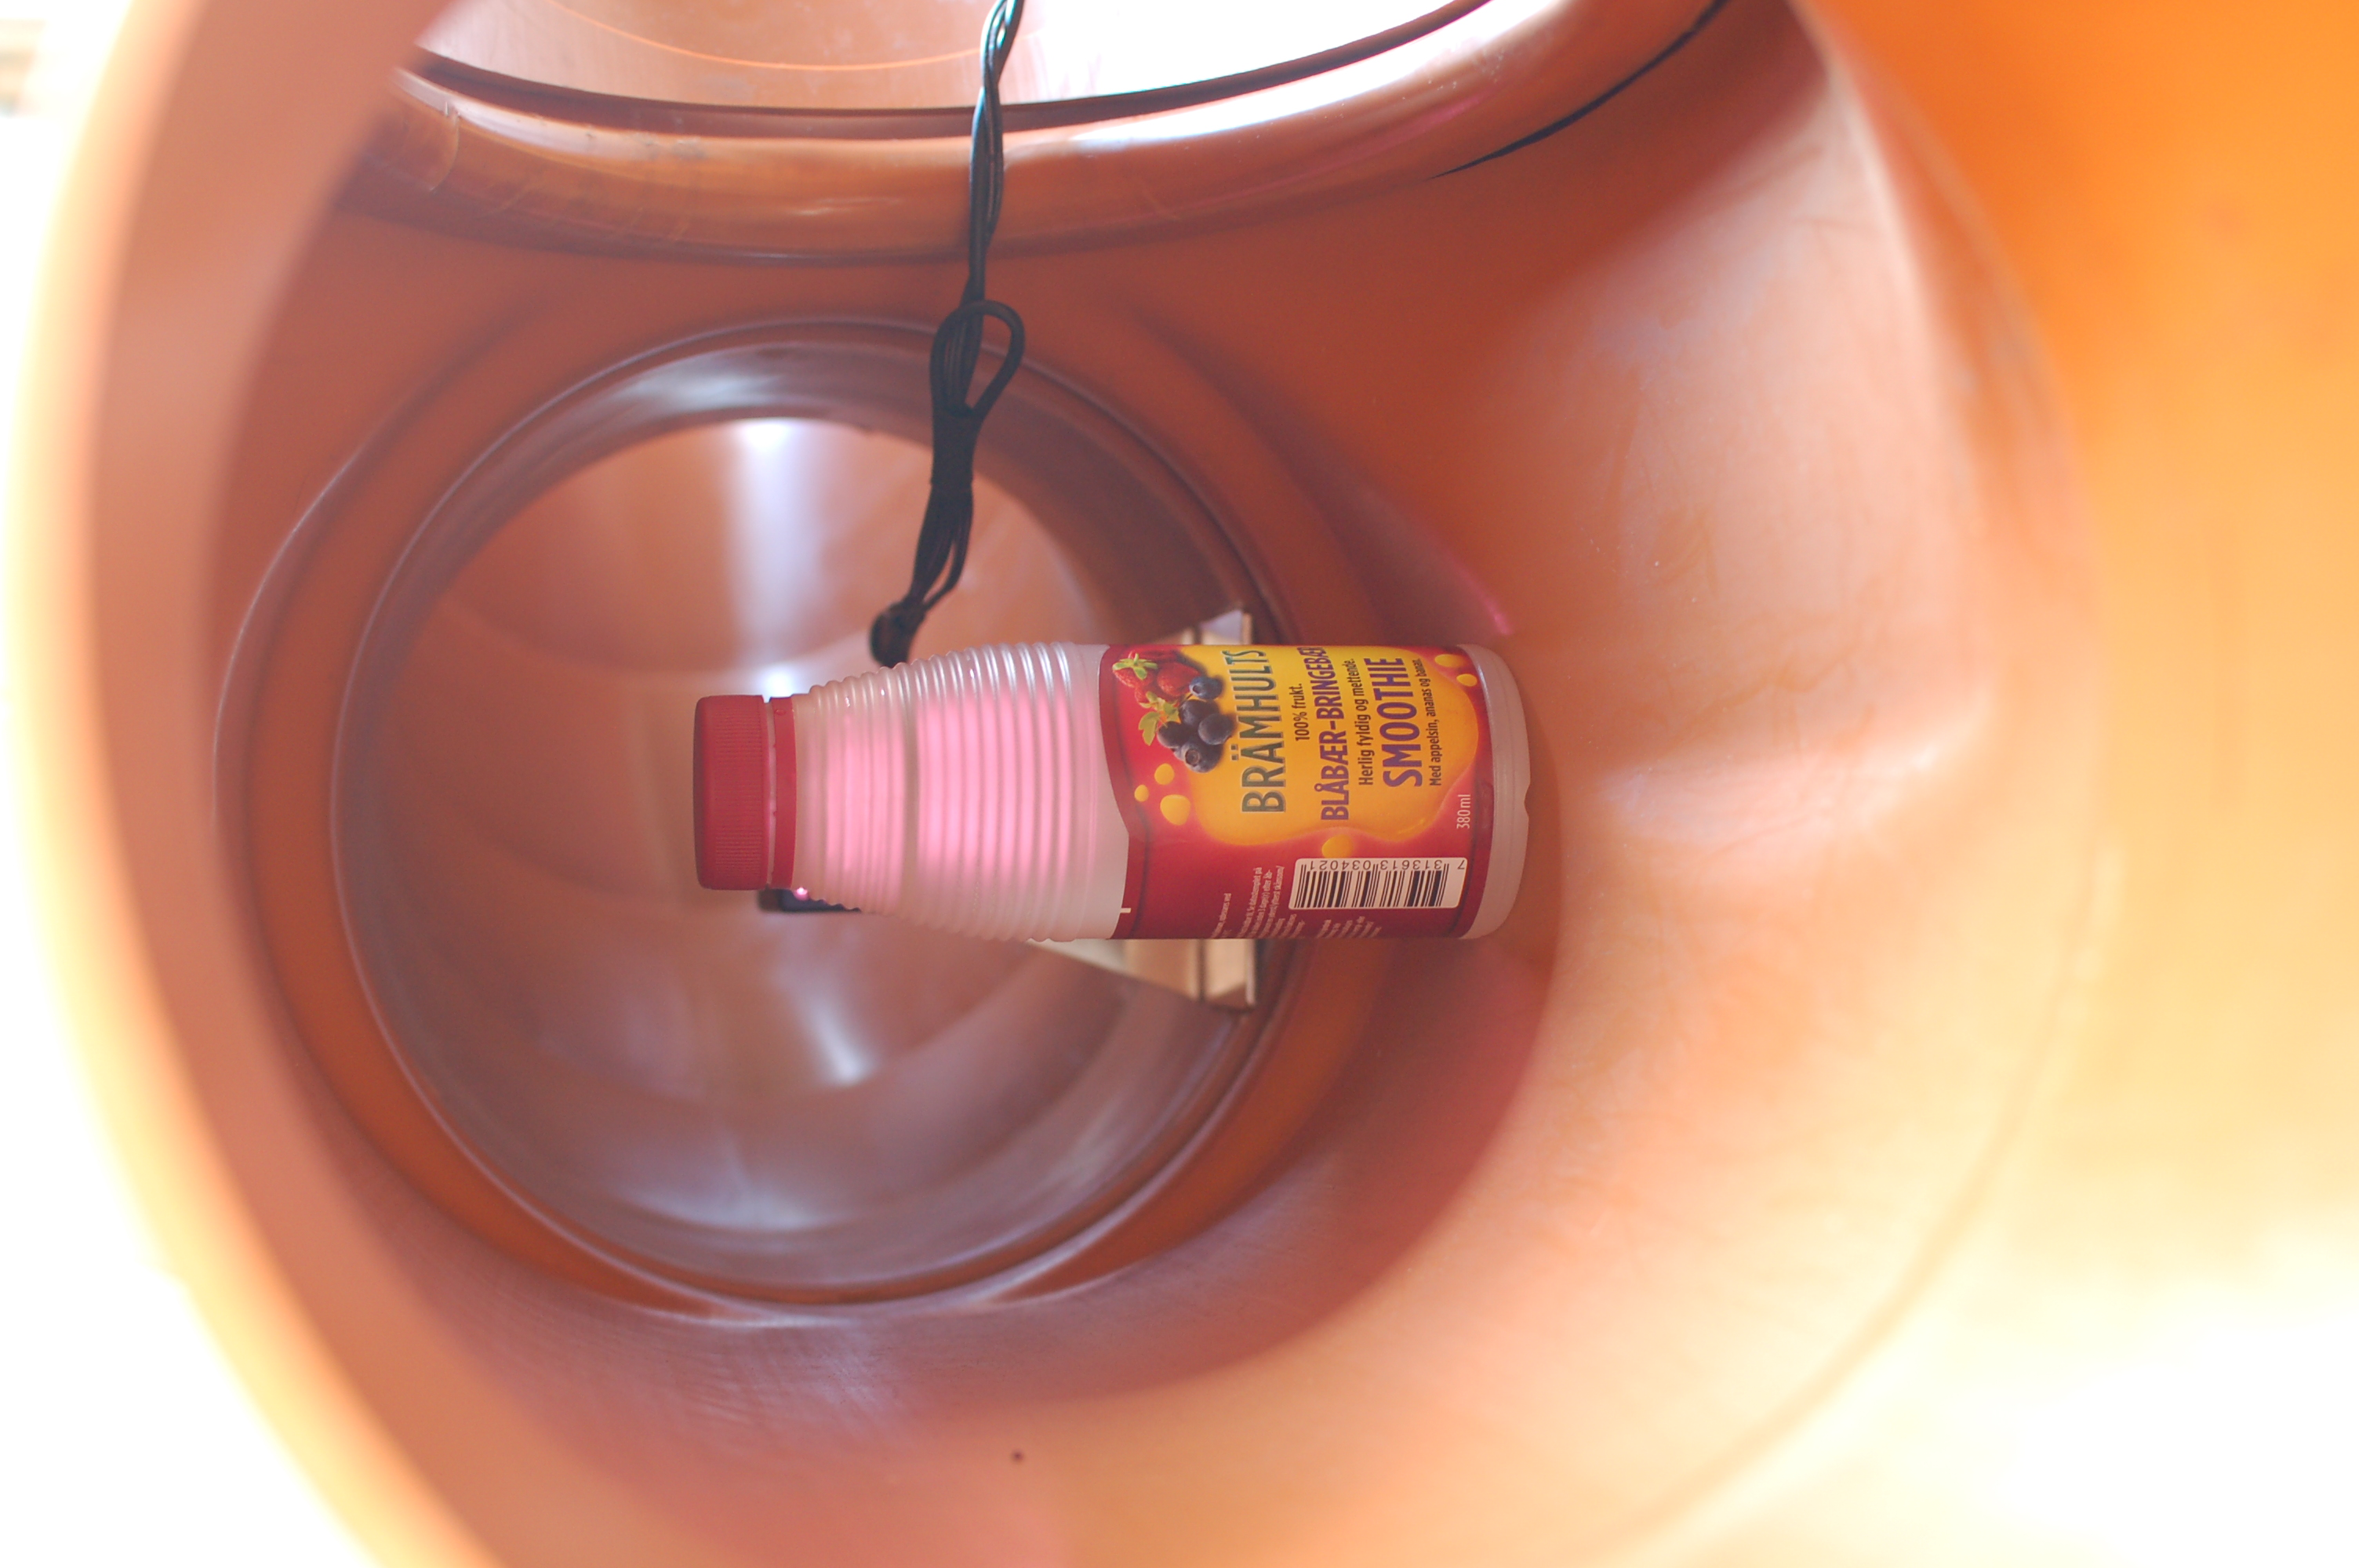
\includegraphics[width=0.47\textwidth]{pics/pos2-regular-tof}
    \caption{Left: The curled-up paper placed at point B in the pipe. Right: Regular
    surfaced obstacle at point B}
    \label{chap7:fig-pics-of-obstacles}
\end{figure}

\subsection{Regular surfaced anomalies}
As mentioned above the algorithm relies on regularity in the environment to detect
anomalies. This test will try to test the ability of the system to detect regular surfaced
objects and how they show up in the sensor output.

In this test an opaque bottle filled with water is placed in the pipe. The right image in Figure
\ref{chap7:fig-pics-of-obstacles} shows the bottle used in the test cases.

\section{Test Results}
The results of the tests are shown here. Only tests show interesting results are given in
this report. 

\subsection{Long Pipe Test at Position One}
Figures \ref{chap7:fig-longpipe-tof-3d}--\ref{chap7:fig-longpipe-urg-2d} shows the test of
the long pipe scenario. Figure \ref{chap7:fig-longpipe-tof-dist} shows the distance from each
point in the data set from the time-of-flight camera to the surface fitted cylinders. The
parameters for this test are shown in Table \ref{chap7:tab-longpipe}. If not otherwise is
stated the parameters are the same for all the tests. 
\begin{table}[htbp]
    \centering
    \begin{tabular}{|c|c|}
        \hline
        Parameter   &   Value   \\
        \hline
        Horizontal Histogram Bin Size & 0.1 \\
        Vertical Histogram Bin Size & 0.5 \\
        Horizontal Point Threshold & 50 \\
        Vertical point Threshold & 30 \\
        \hline
        Cylinder fit Interval & 0.3 \\
        Low-intensity Threshold & 500 \\
        High-intensity Threshold & 15 000 \\
        \hline
        Parallel line threshold & 0.01 \\
        \hline
    \end{tabular}
    \caption{Test parameters for the long pipe test}
    \label{chap7:tab-longpipe}
\end{table}
\begin{figure}[htbp]
    \centering
    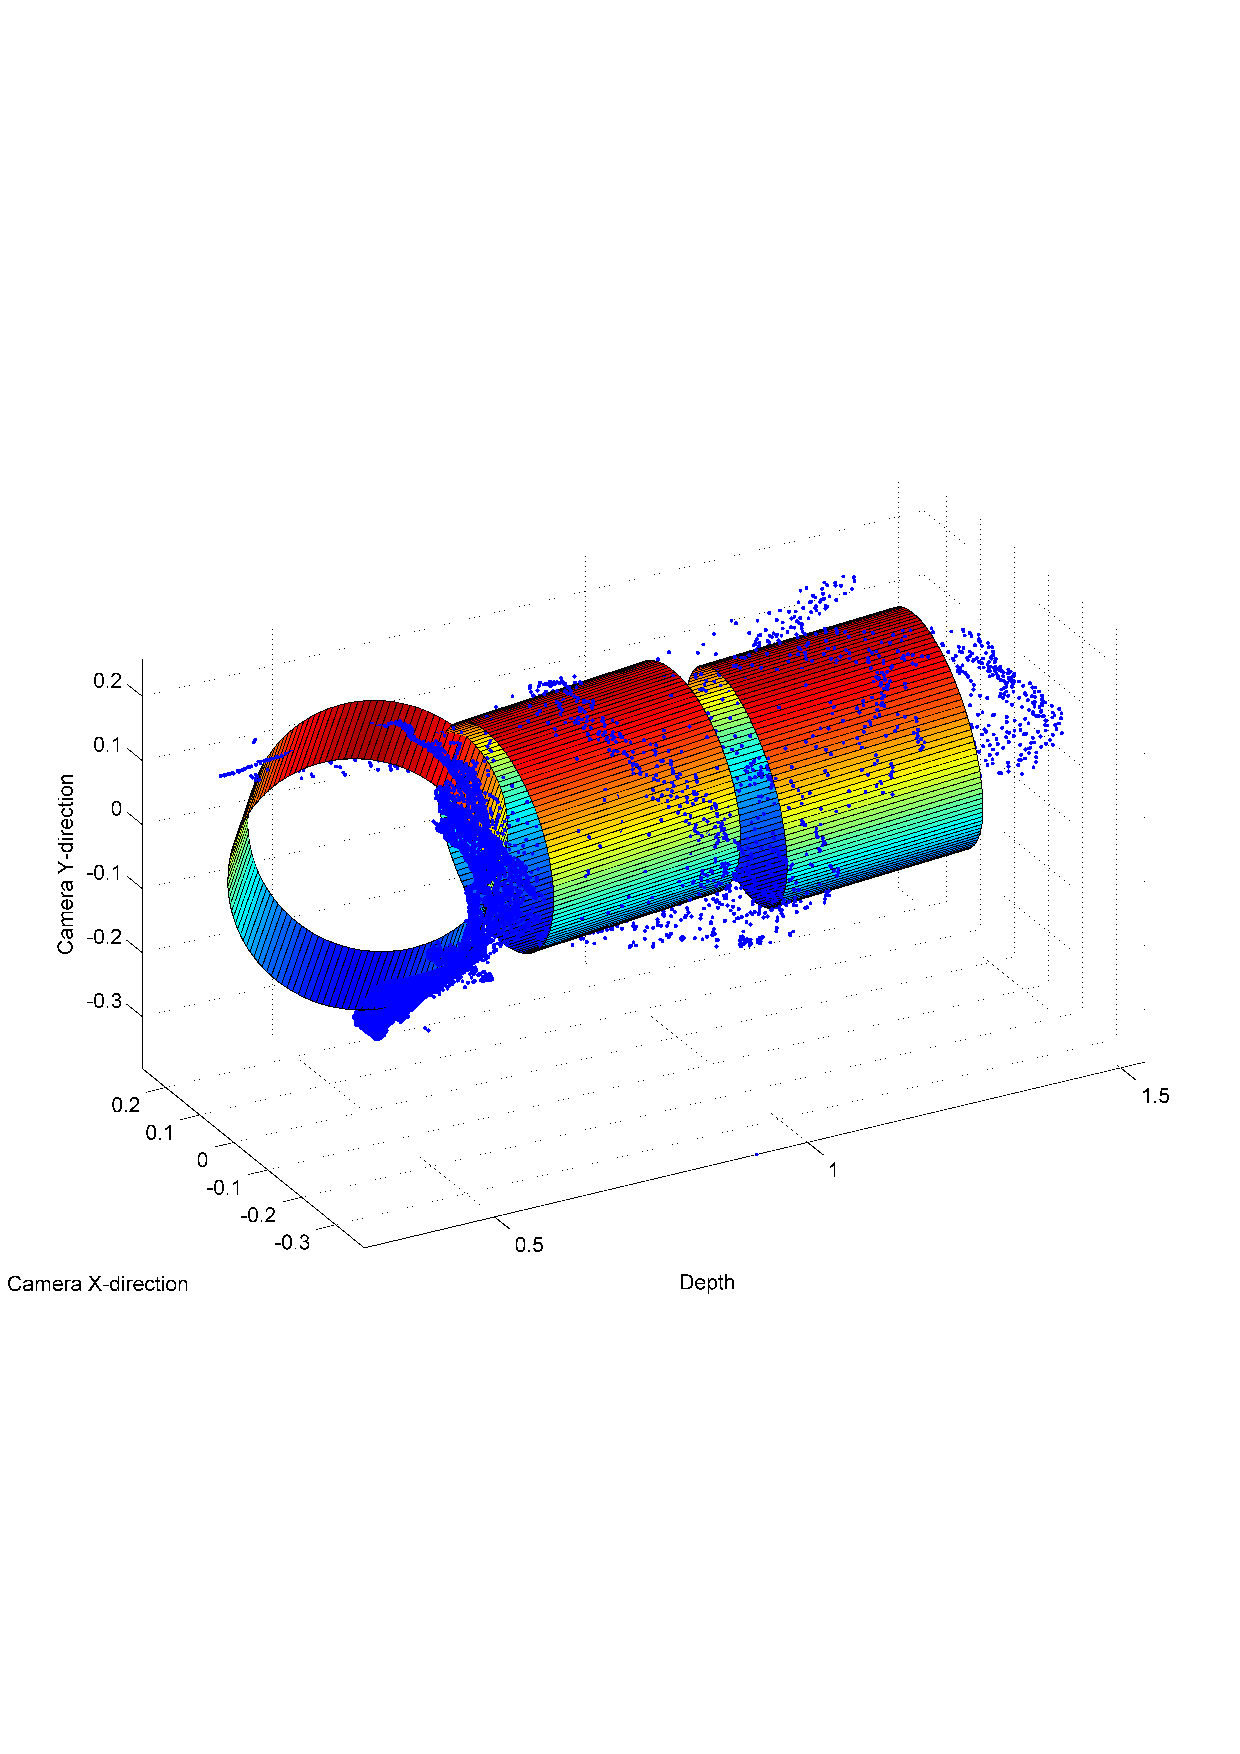
\includegraphics[width=0.8\textwidth]{pics/longpipe-tof-3d}
    \caption{The point cloud and fitted cylinders taken from the time-of-flight camera for
    the long pipe test.}
    \label{chap7:fig-longpipe-tof-3d}
\end{figure}
\begin{figure}[htbp]
    \centering
    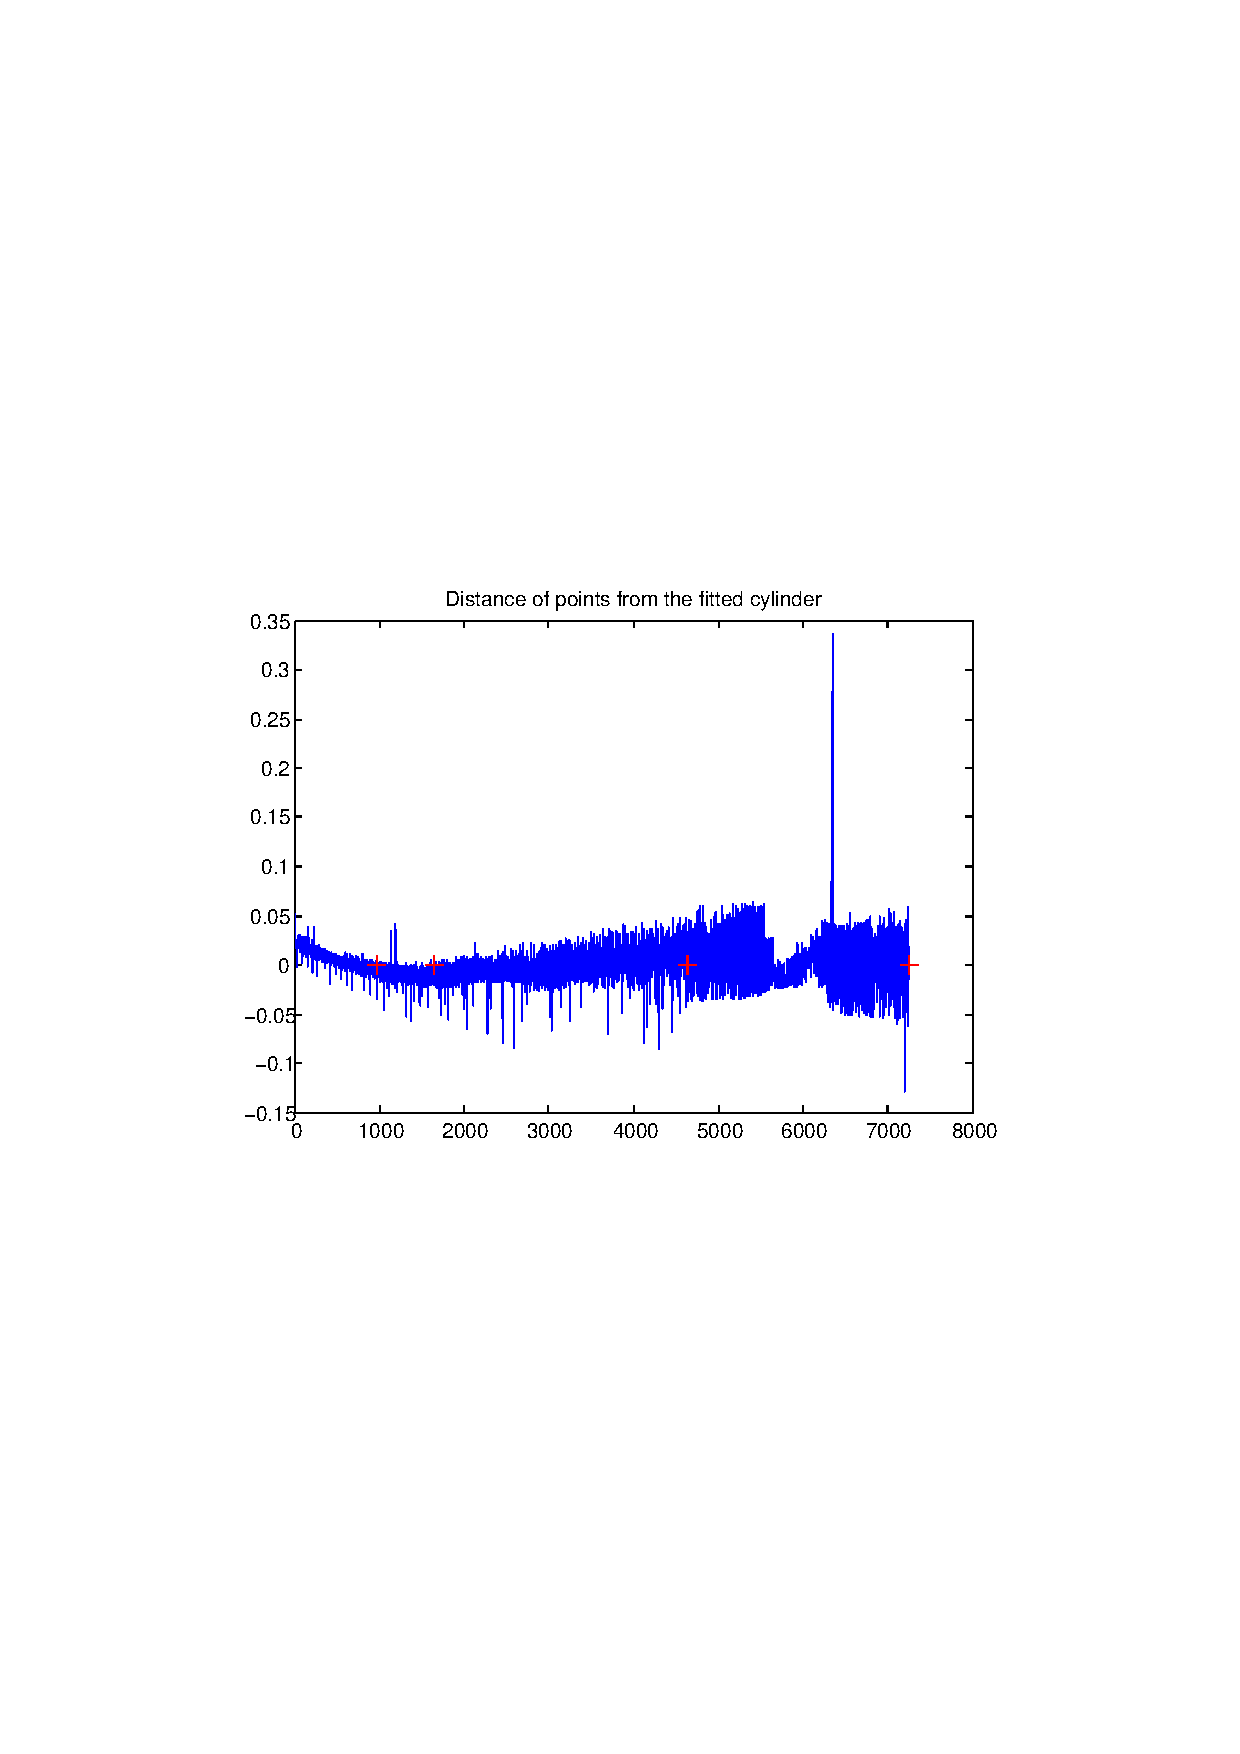
\includegraphics[width=0.8\textwidth]{pics/longpipe-tof-dist}
    \caption{The distance of the points from the fitted cylinders at position 1 for the
    long pipe test}
    \label{chap7:fig-longpipe-tof-dist}
\end{figure}
\begin{figure}[htbp]
    \centering
    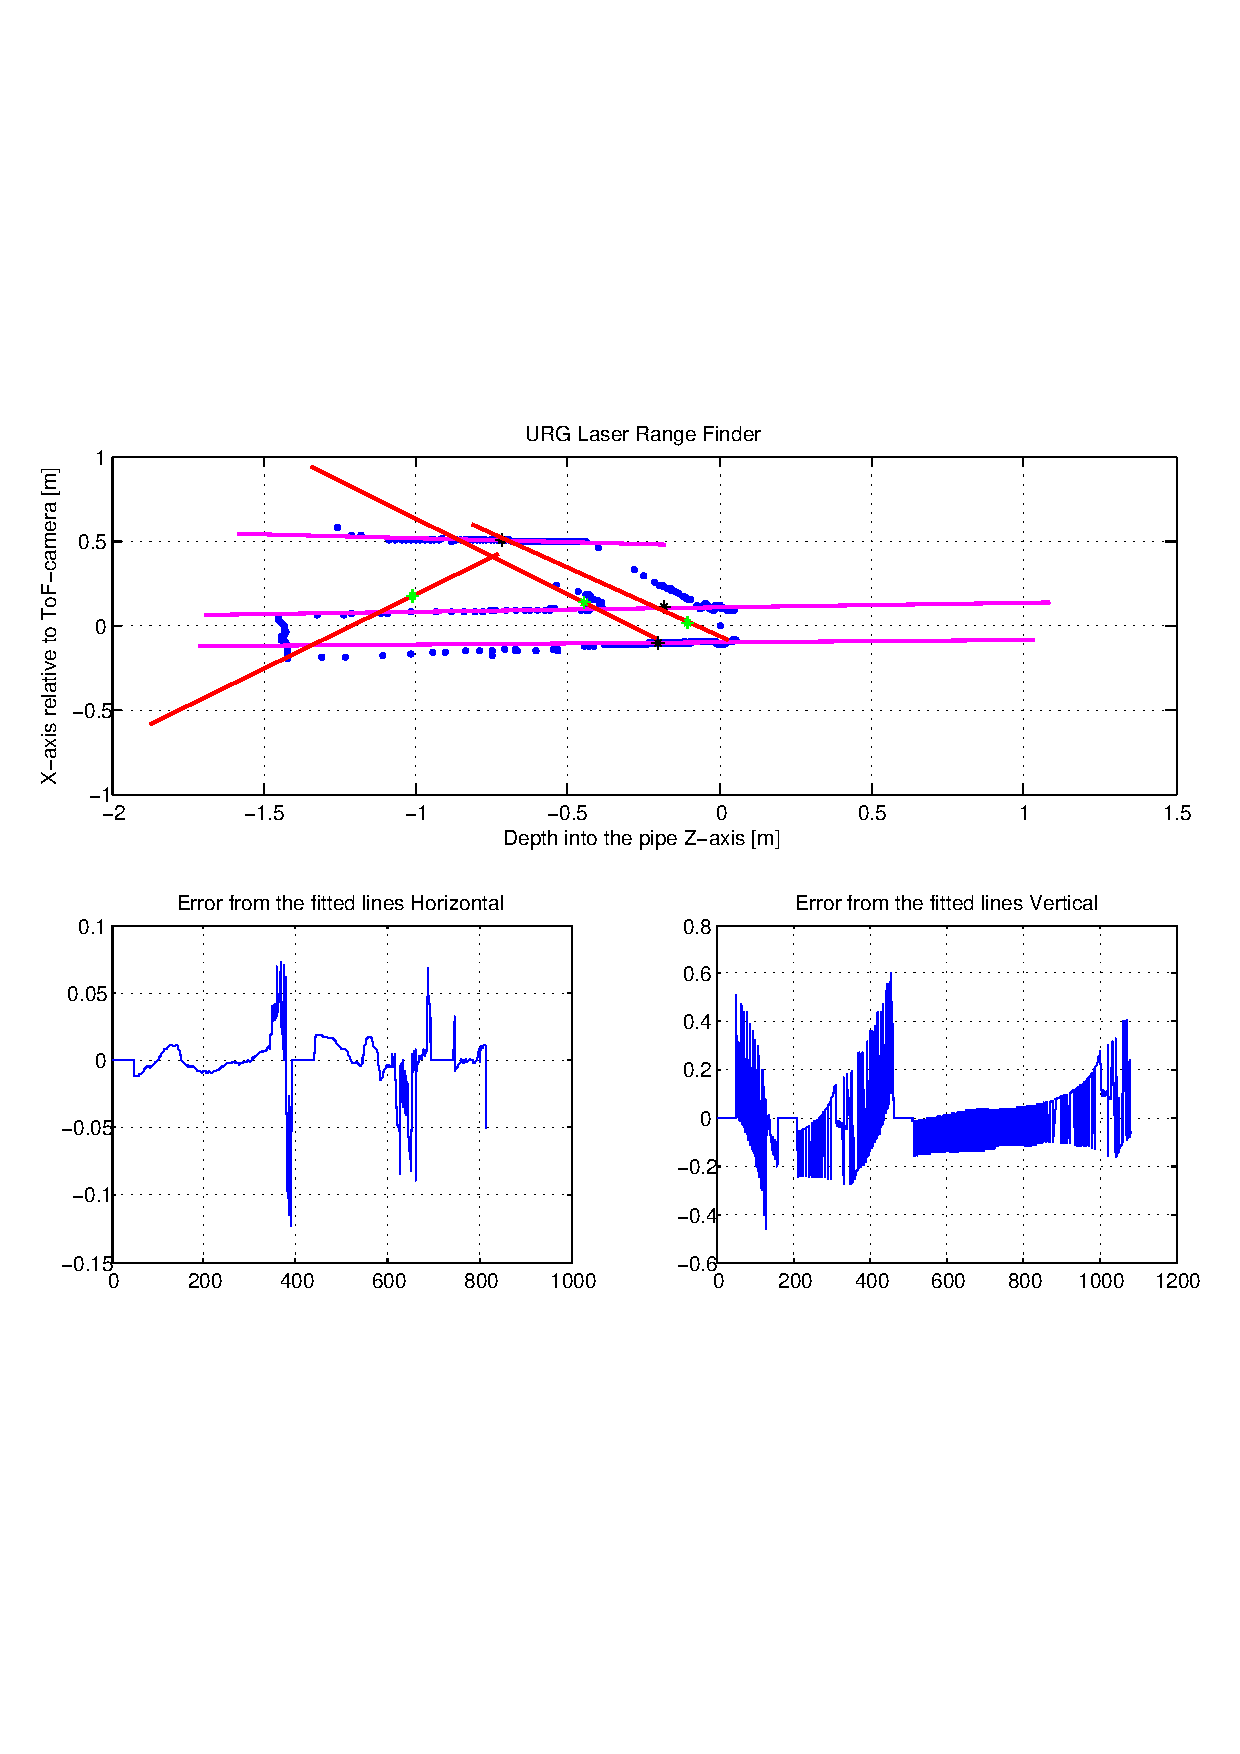
\includegraphics[width=0.8\textwidth]{pics/longpipe-urg-2d}
    \caption{The data from the URG Laser Range Finder with fitted lines at position 1 for
    the long pipe test}
    \label{chap7:fig-longpipe-urg-2d}
\end{figure}

\subsection{Control Case at Position Two Looking at the $90^\circ$ R- bend}
This test shows how the algorithms perform in the ideal case when placed inside the
pipe. The parameters were the same as for the long pipe test. See Fiugres
\ref{chap7:fig-pos21-control-tof-3d}--\ref{chap7:fig-pos21-control-urg-2d}.
\begin{figure}[htbp]
    \centering
    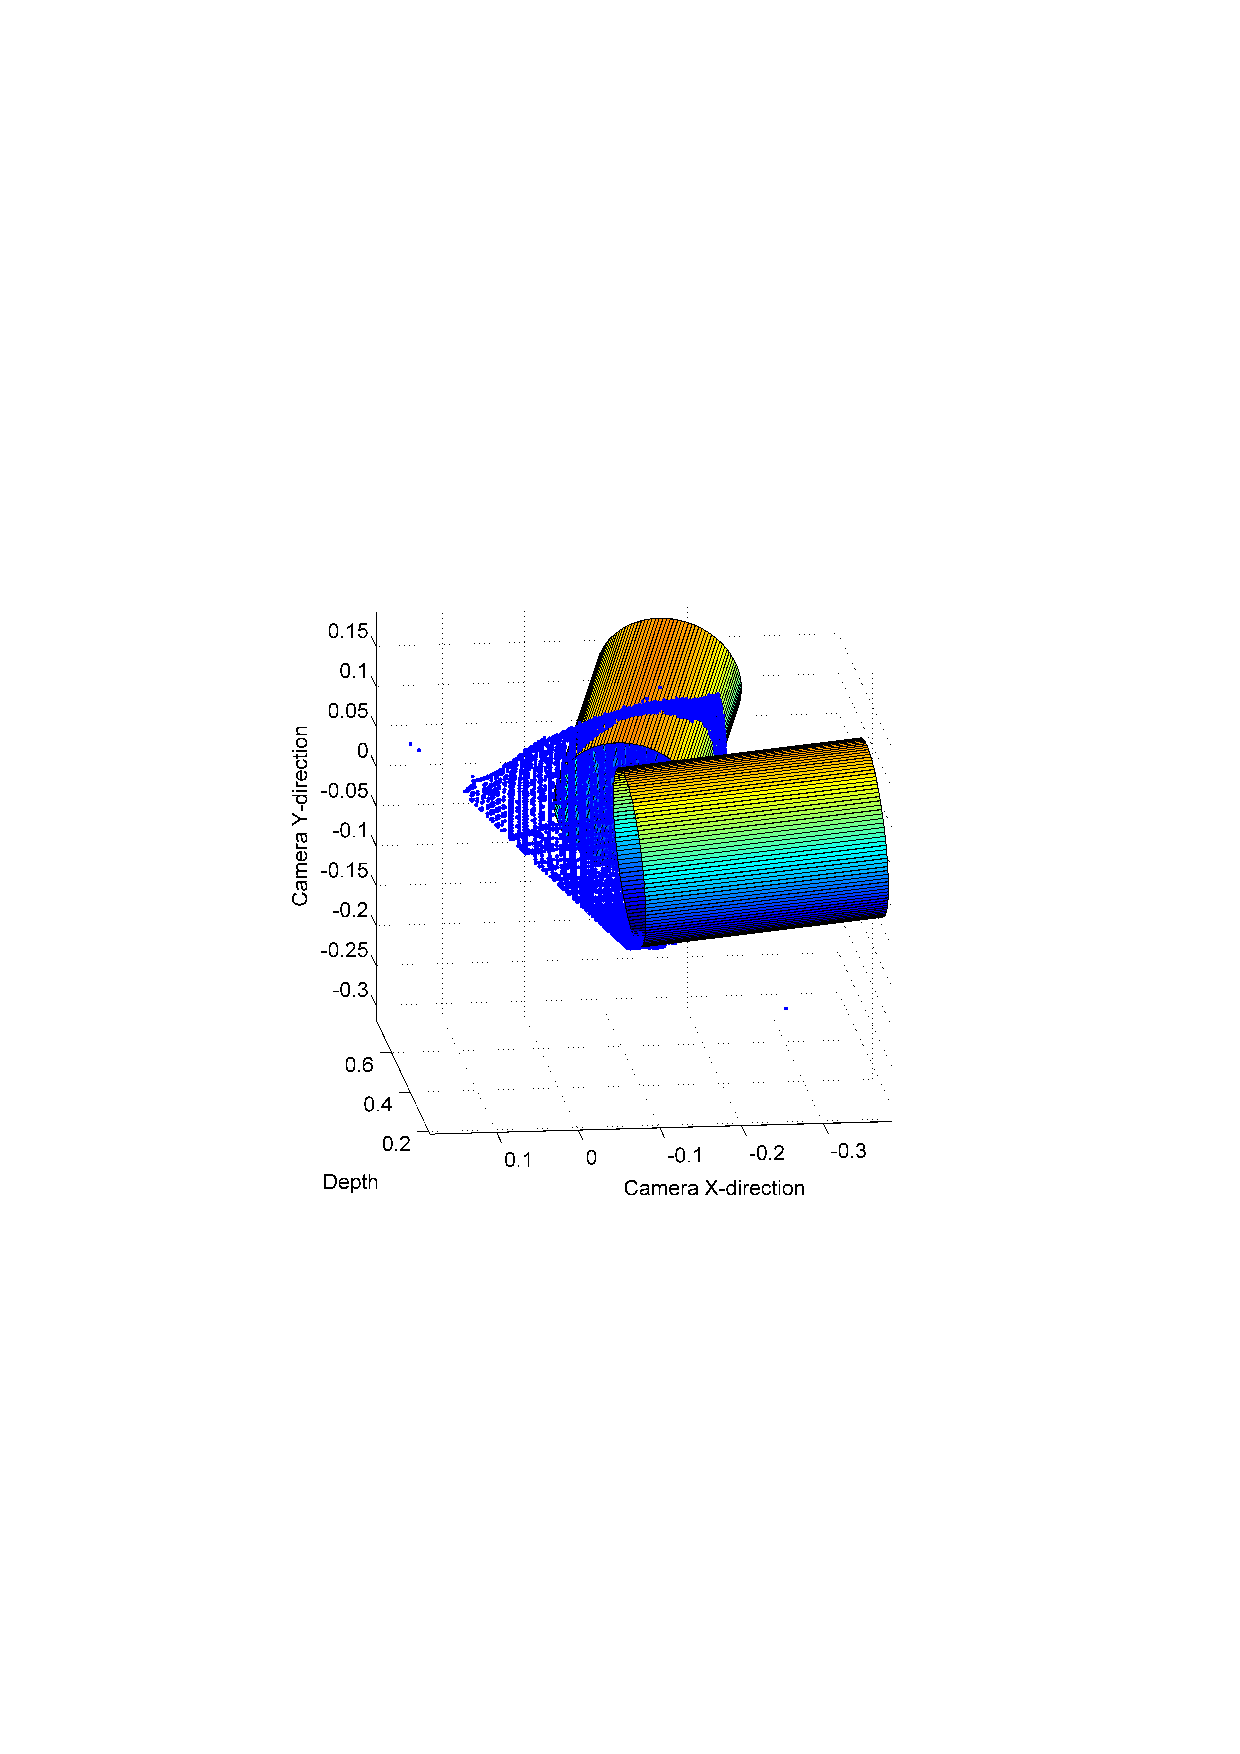
\includegraphics[width=0.7\textwidth]{pics/pos21-control-tof-3d}
    \caption{The point cloud and fitted cylinders taken from the time-of-flight camera at
    position 2}
    \label{chap7:fig-pos21-control-tof-3d}
\end{figure}
\begin{figure}[htbp]
    \centering
    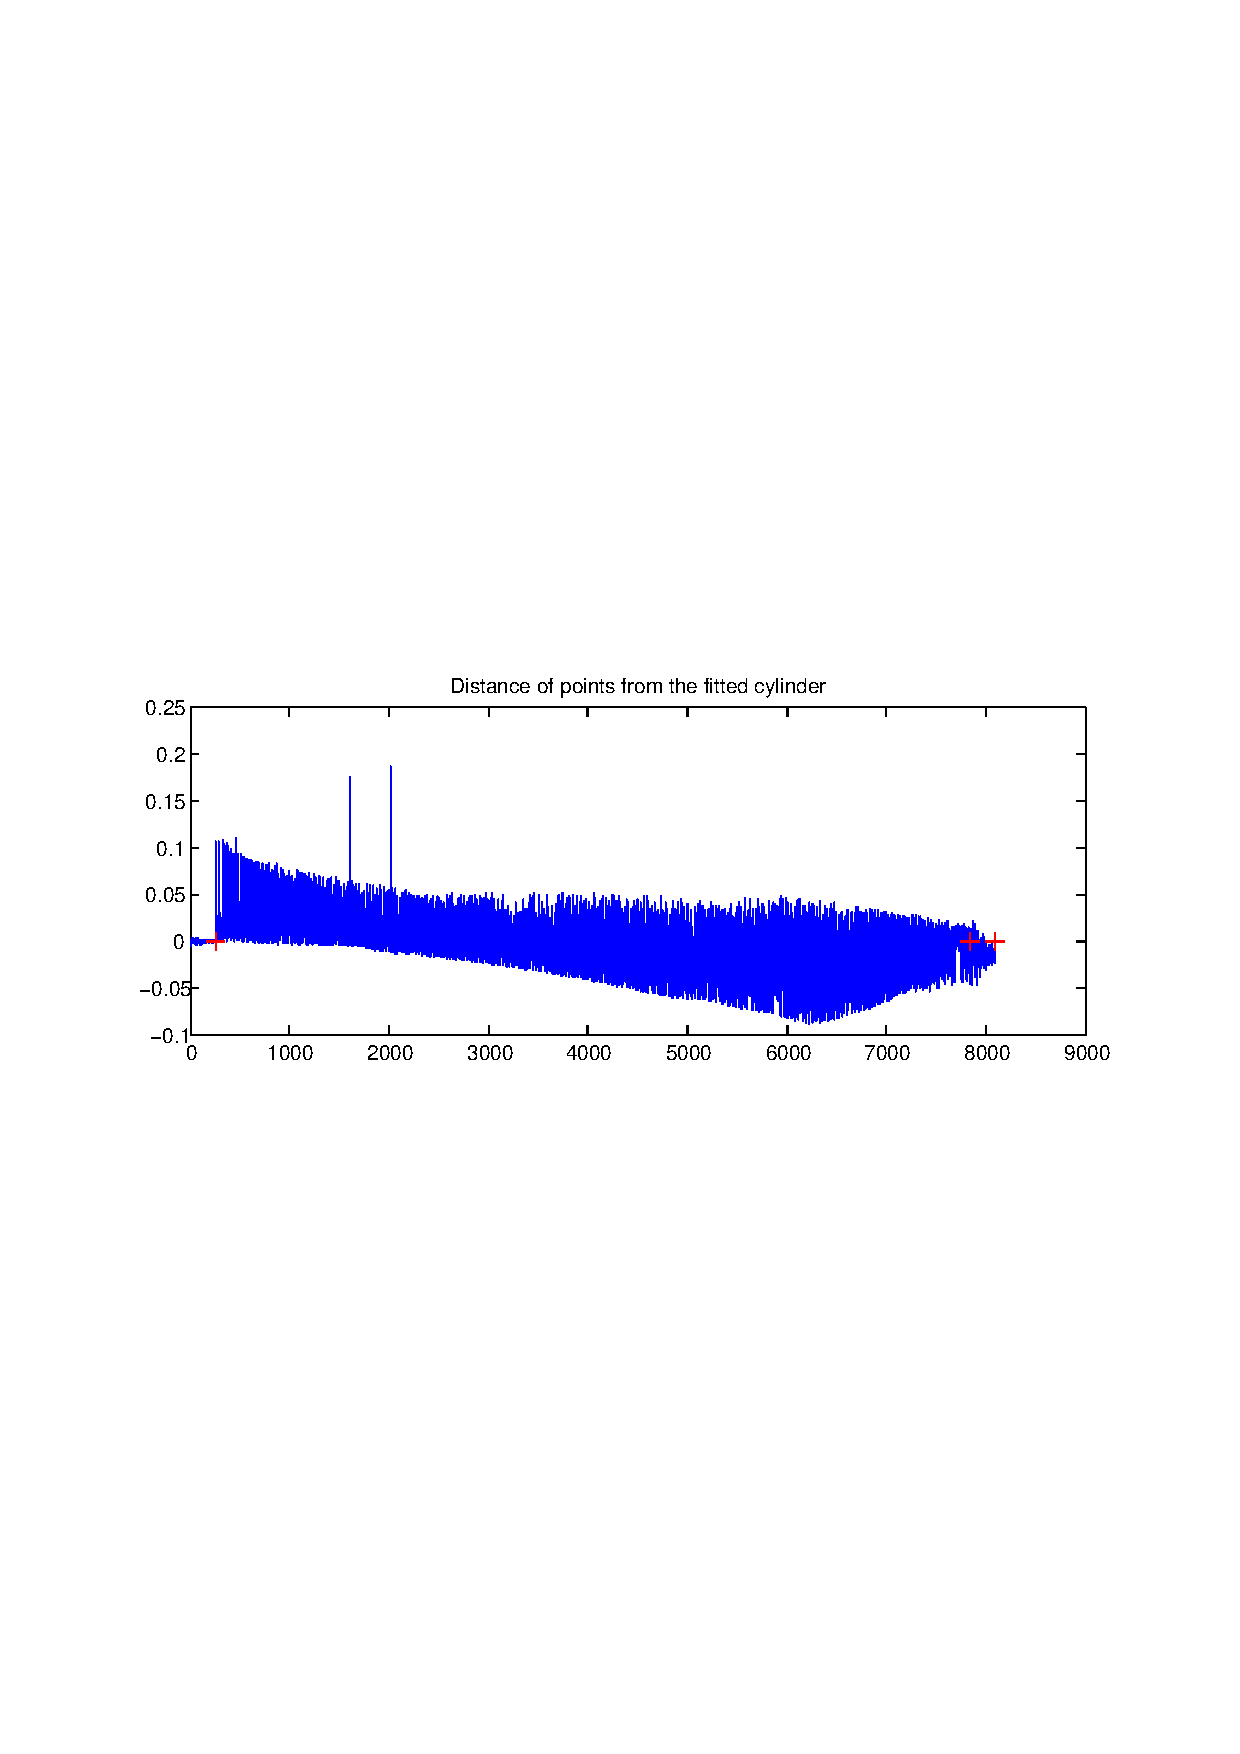
\includegraphics[width=0.9\textwidth]{pics/pos21-control-tof-dist}
    \caption{The distance of the points from the fitted cylinders at position 2}
    \label{chap7:fig-pos21-control-tof-dits}
\end{figure}
\begin{figure}[htbp]
    \centering
    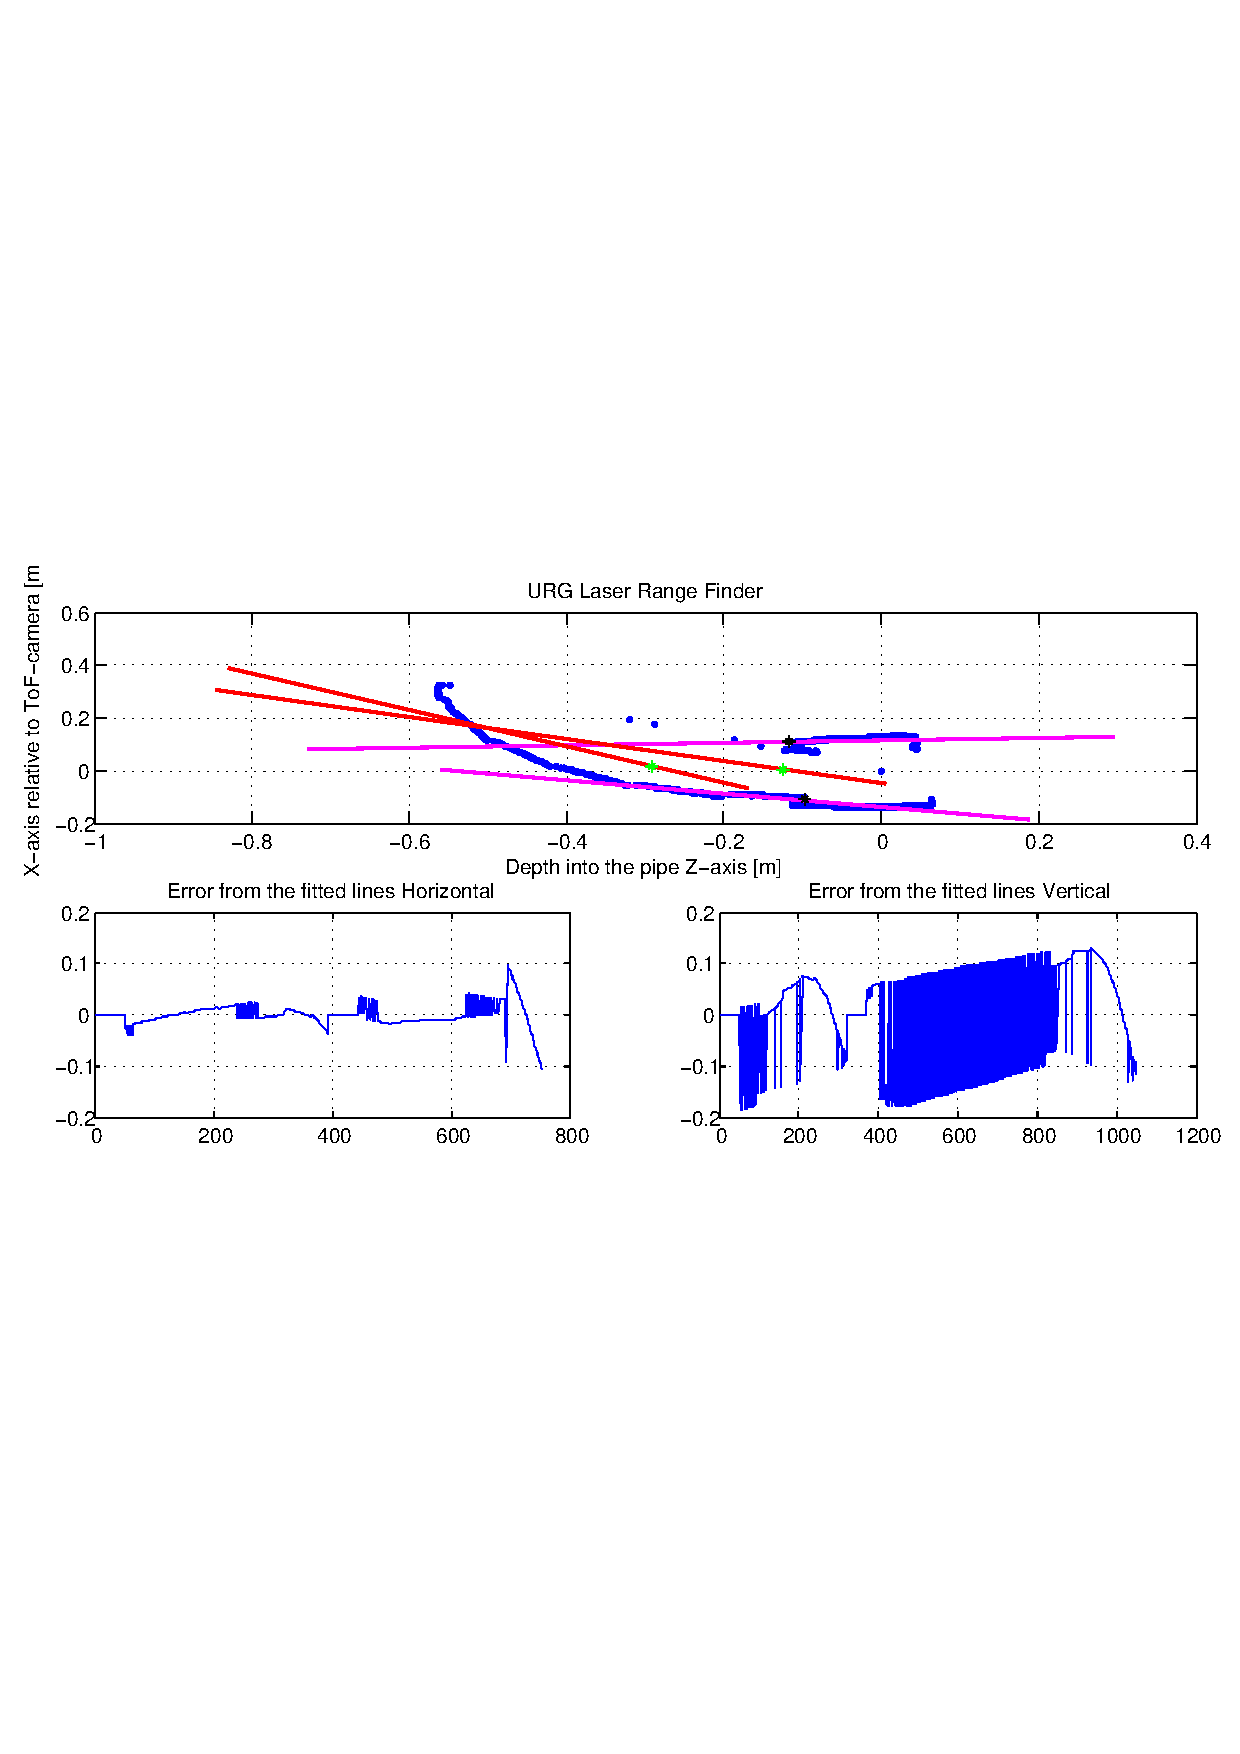
\includegraphics[width=0.9\textwidth]{pics/pos21-control-urg-2d}
    \caption{The data from the URG Laser Range Finder with fitted lines at position 2}
    \label{chap7:fig-pos21-control-urg-2d}
\end{figure}


\subsection{Irregular test at Position Two Looking at position one}
This plots show how an open end of a pipe shows up in the sensors. The outside of the
pipeline is quite structured, and the camera gives disparity images from the outside of
the pipe. Figures
\ref{chap7:fig-pos2-irregular-tof-3d}-\ref{chap7:fig-pos2-irregular-rectified} shows the
results from the test. 
\begin{figure}[htbp]
    \centering
    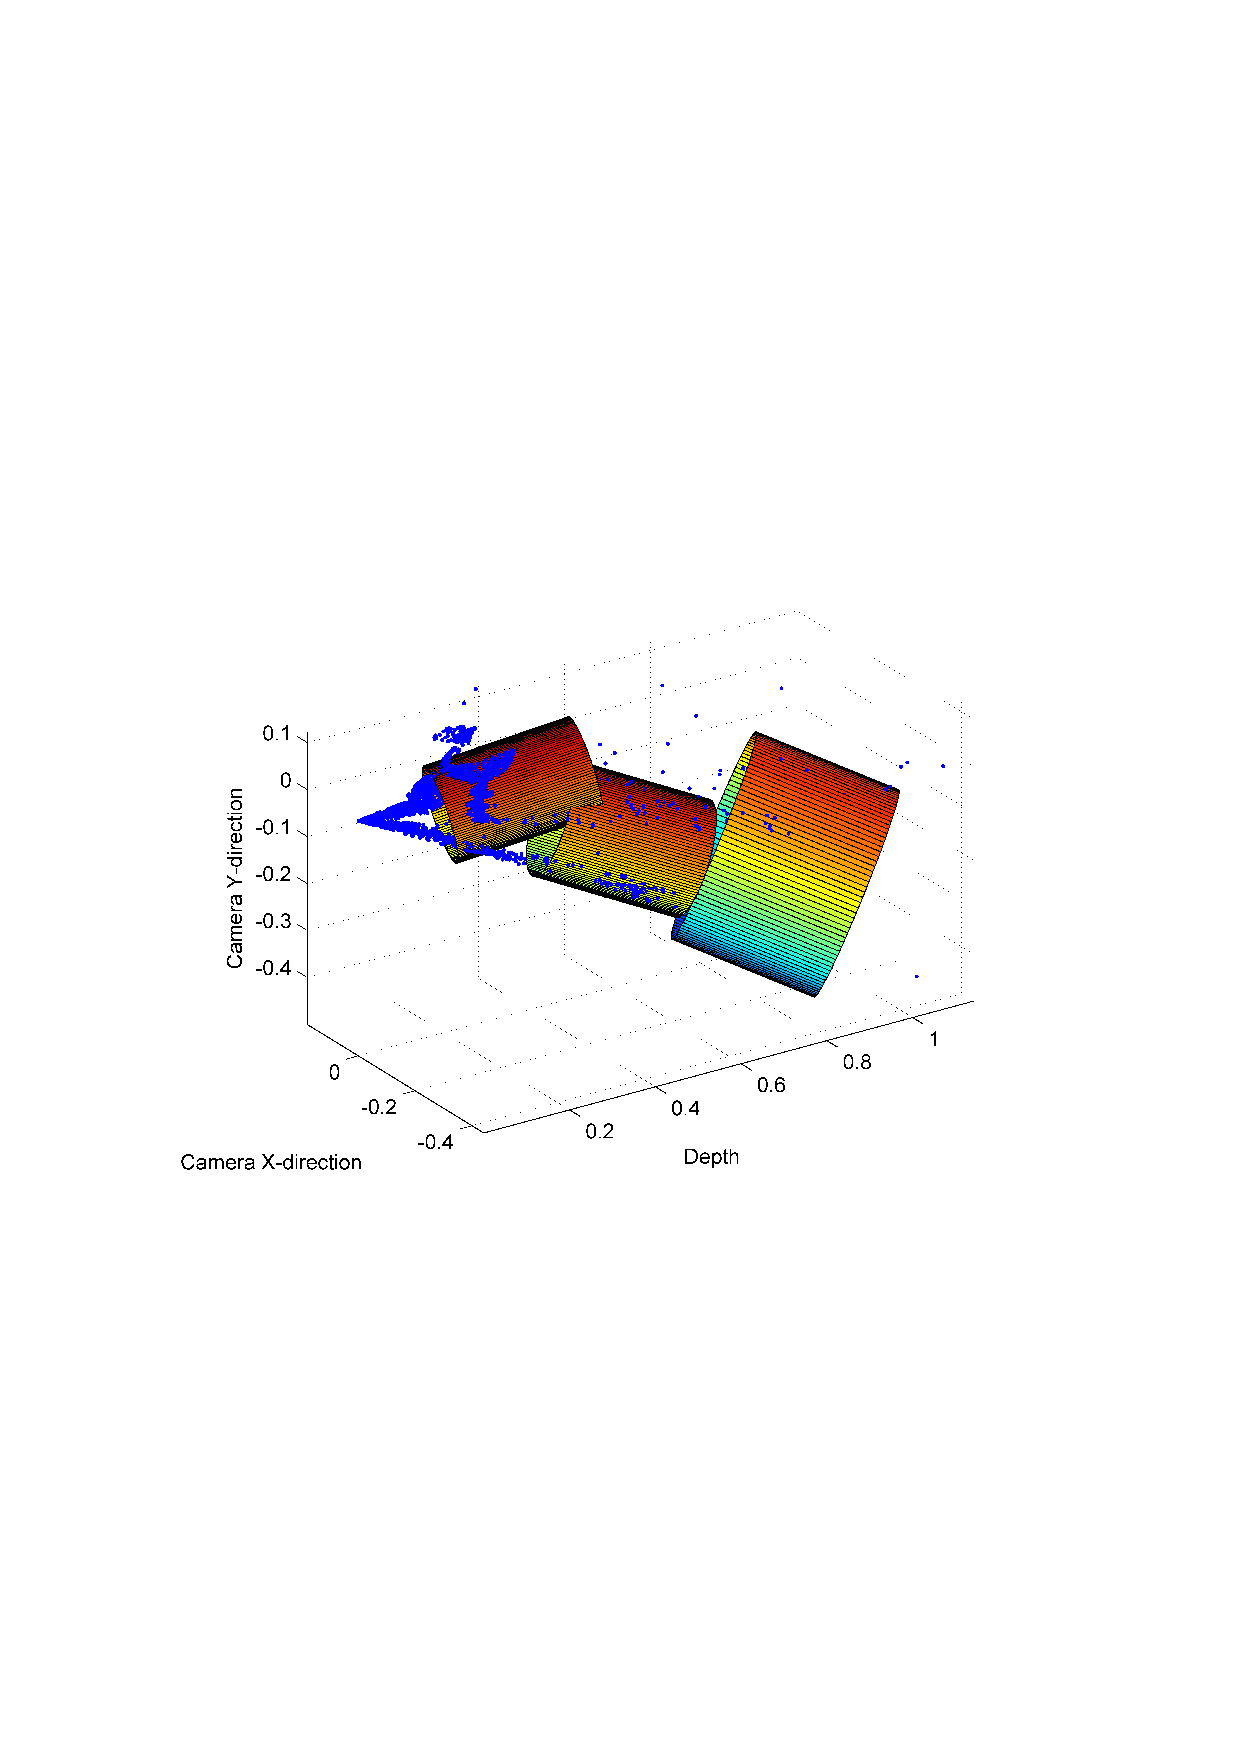
\includegraphics[width=0.7\textwidth]{pics/pos2-irregular-tof-3d}
    \caption{The point cloud and fitted cylinders taken from the time-of-flight camera at
    position 2}
    \label{chap7:fig-pos2-irregular-tof-3d}
\end{figure}
\begin{figure}[htbp]
    \centering
    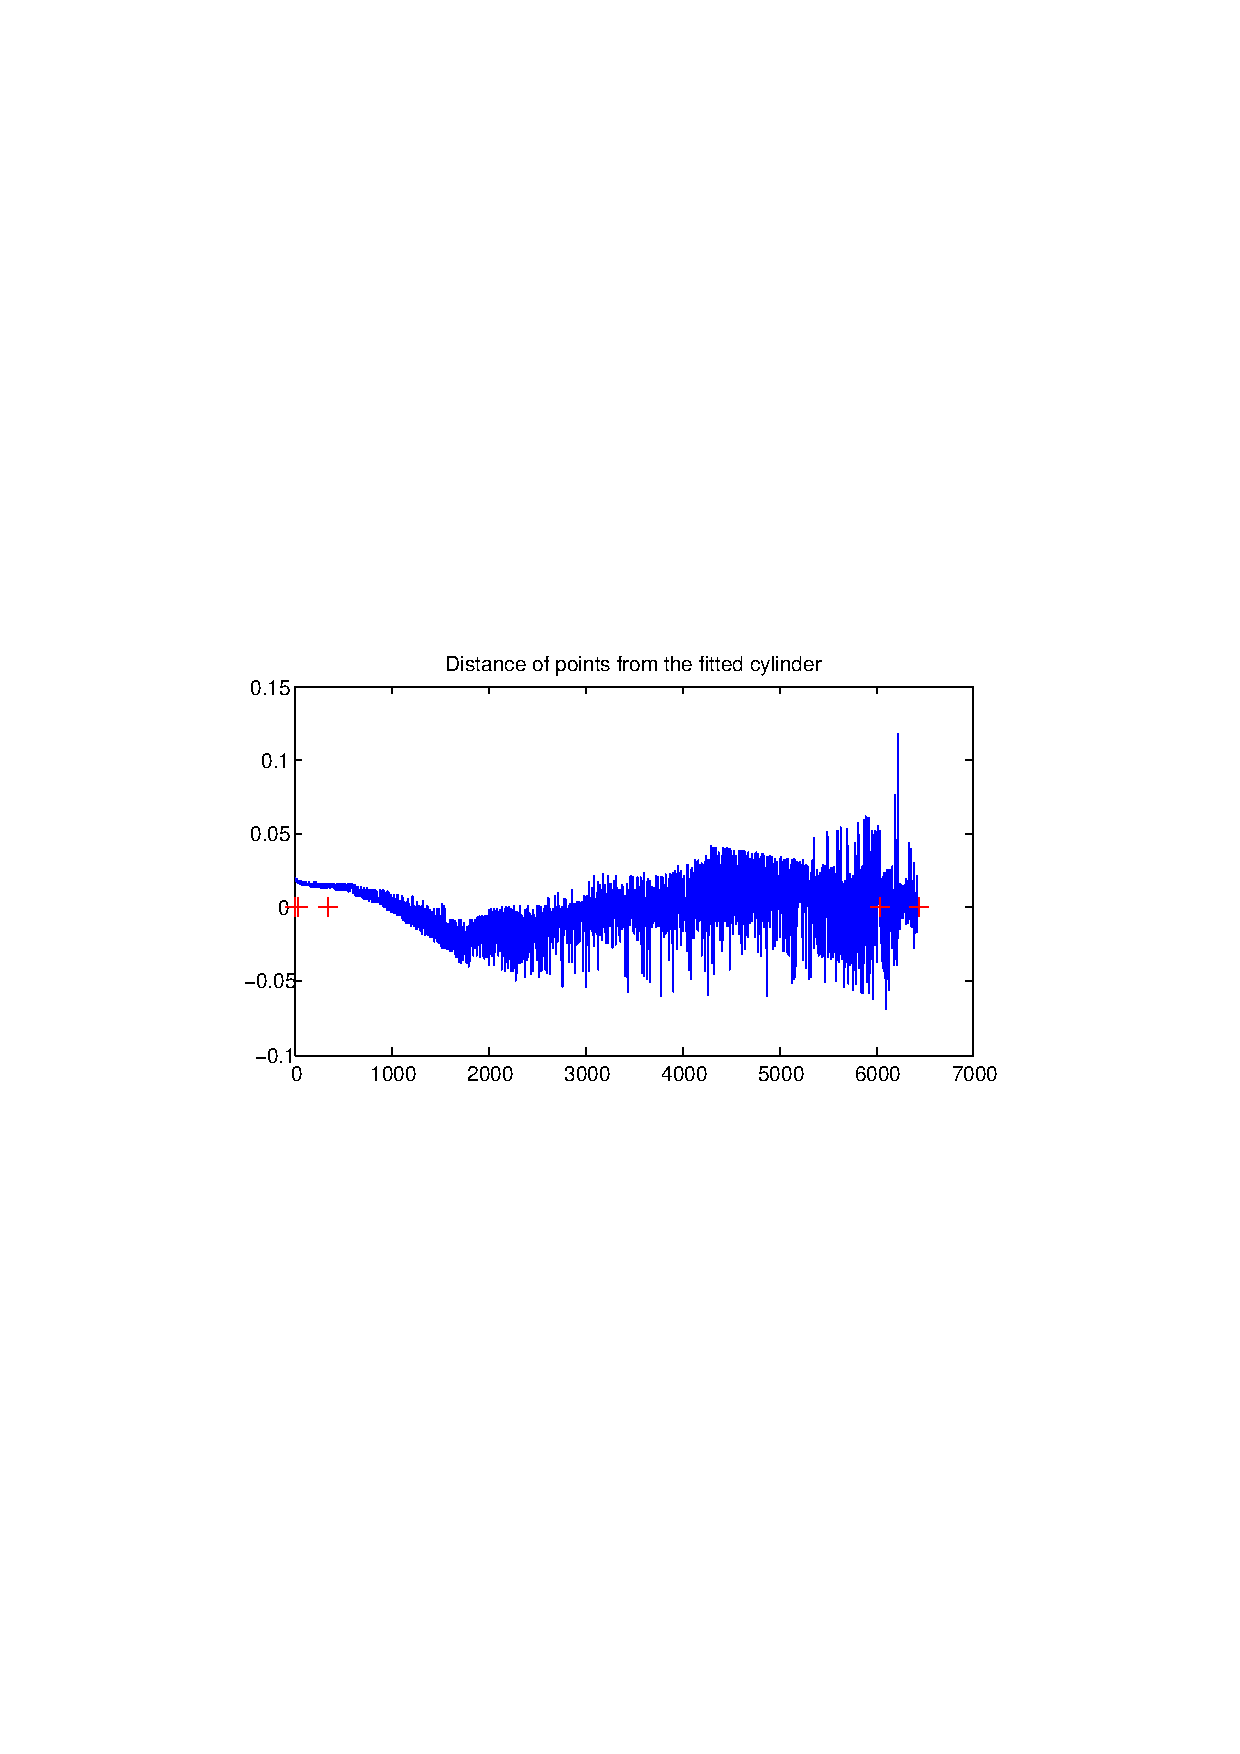
\includegraphics[width=0.9\textwidth]{pics/pos2-irregular-tof-dist}
    \caption{The distance of the points from the fitted cylinders at position 2 looking at
    position 1}
    \label{chap7:fig-pos2-irregular-tof-dits}
\end{figure}
\begin{figure}[htbp]
    \centering
    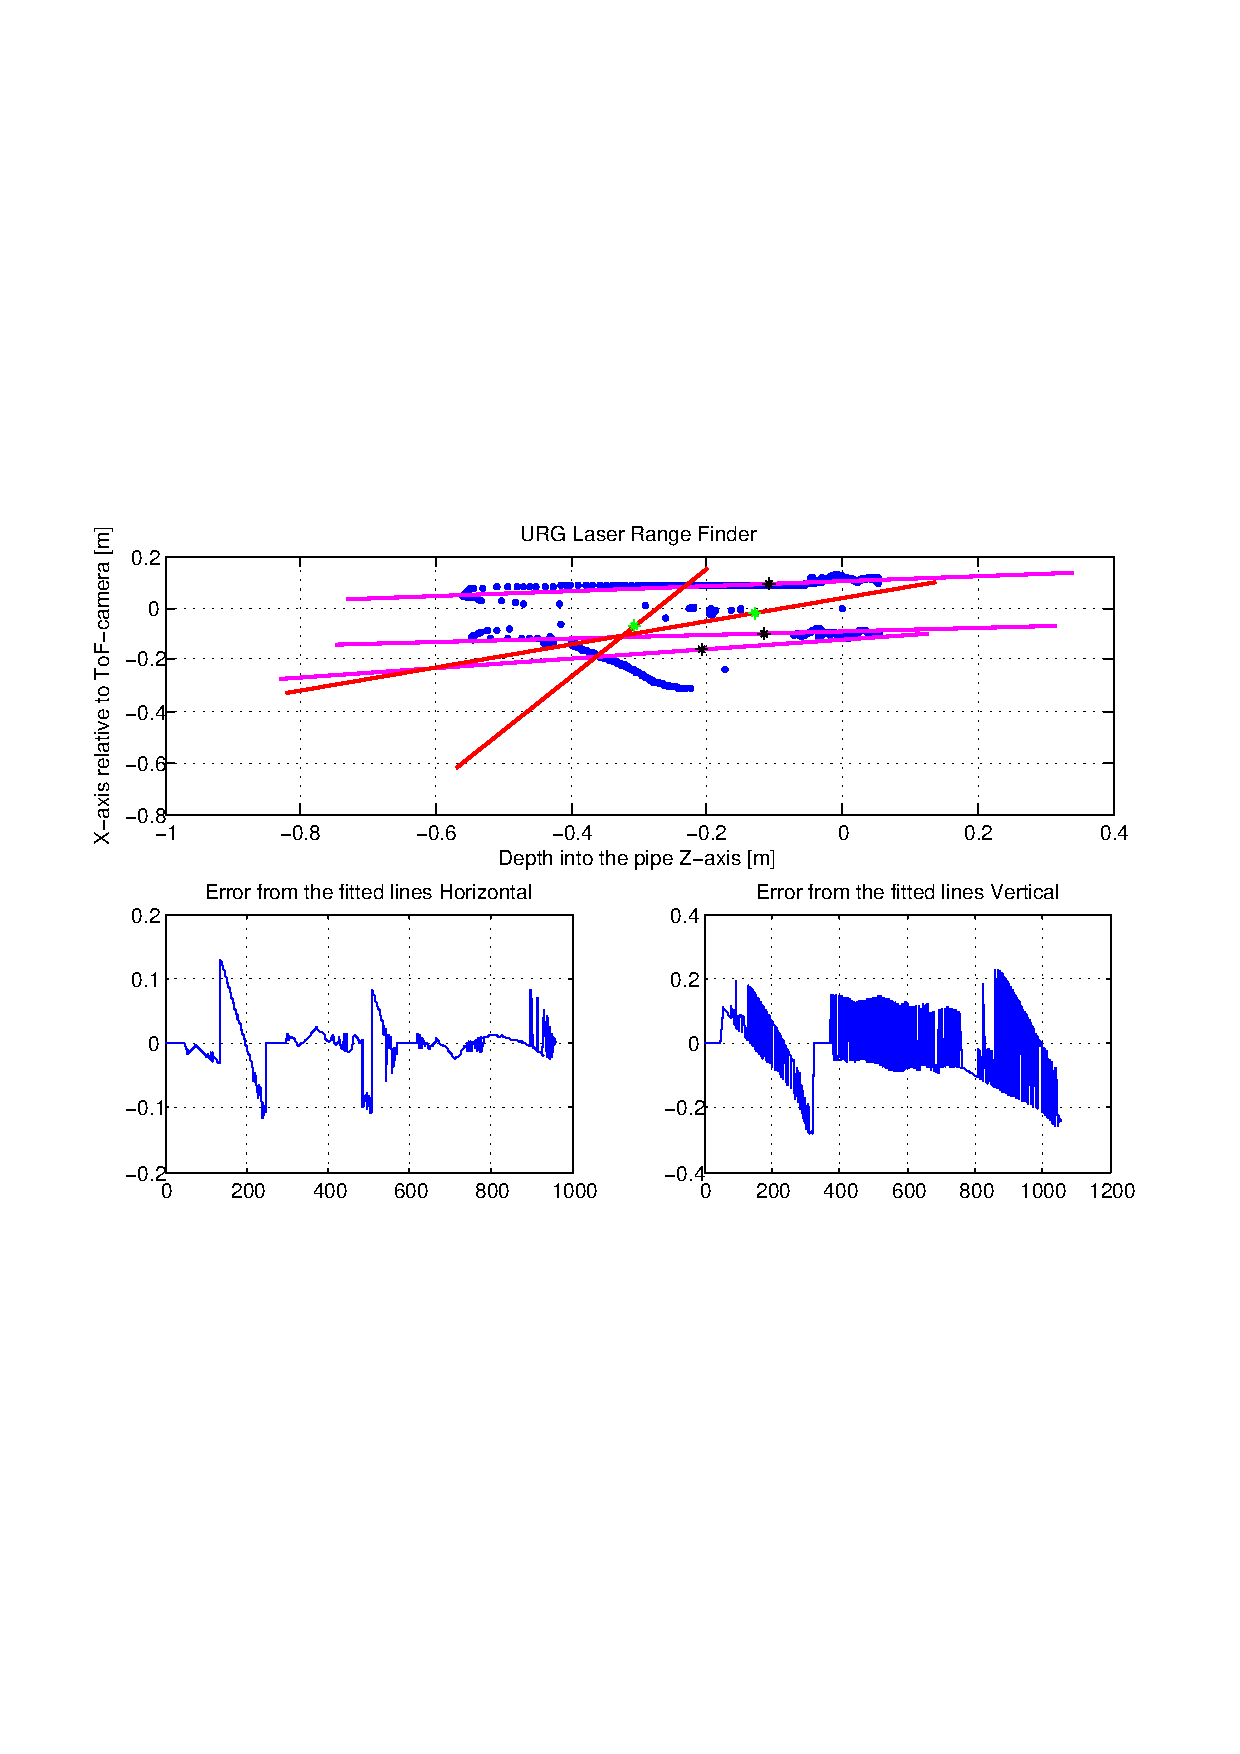
\includegraphics[width=0.9\textwidth]{pics/pos2-irregular-urg-2d}
    \caption{The data from the URG Laser Range Finder with fitted lines at position 2
    looking at position 1}
    \label{chap7:fig-pos2-irregular-urg-2d}
\end{figure}
\begin{figure}[htbp]
    \centering
    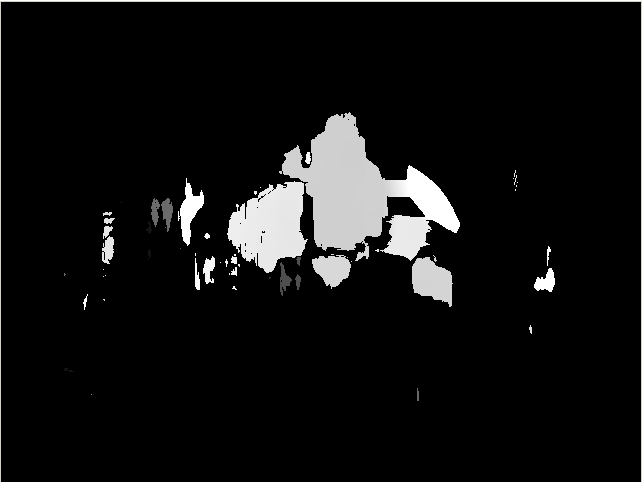
\includegraphics[width=0.37\textwidth]{pics/pos2-irregular-depth}
    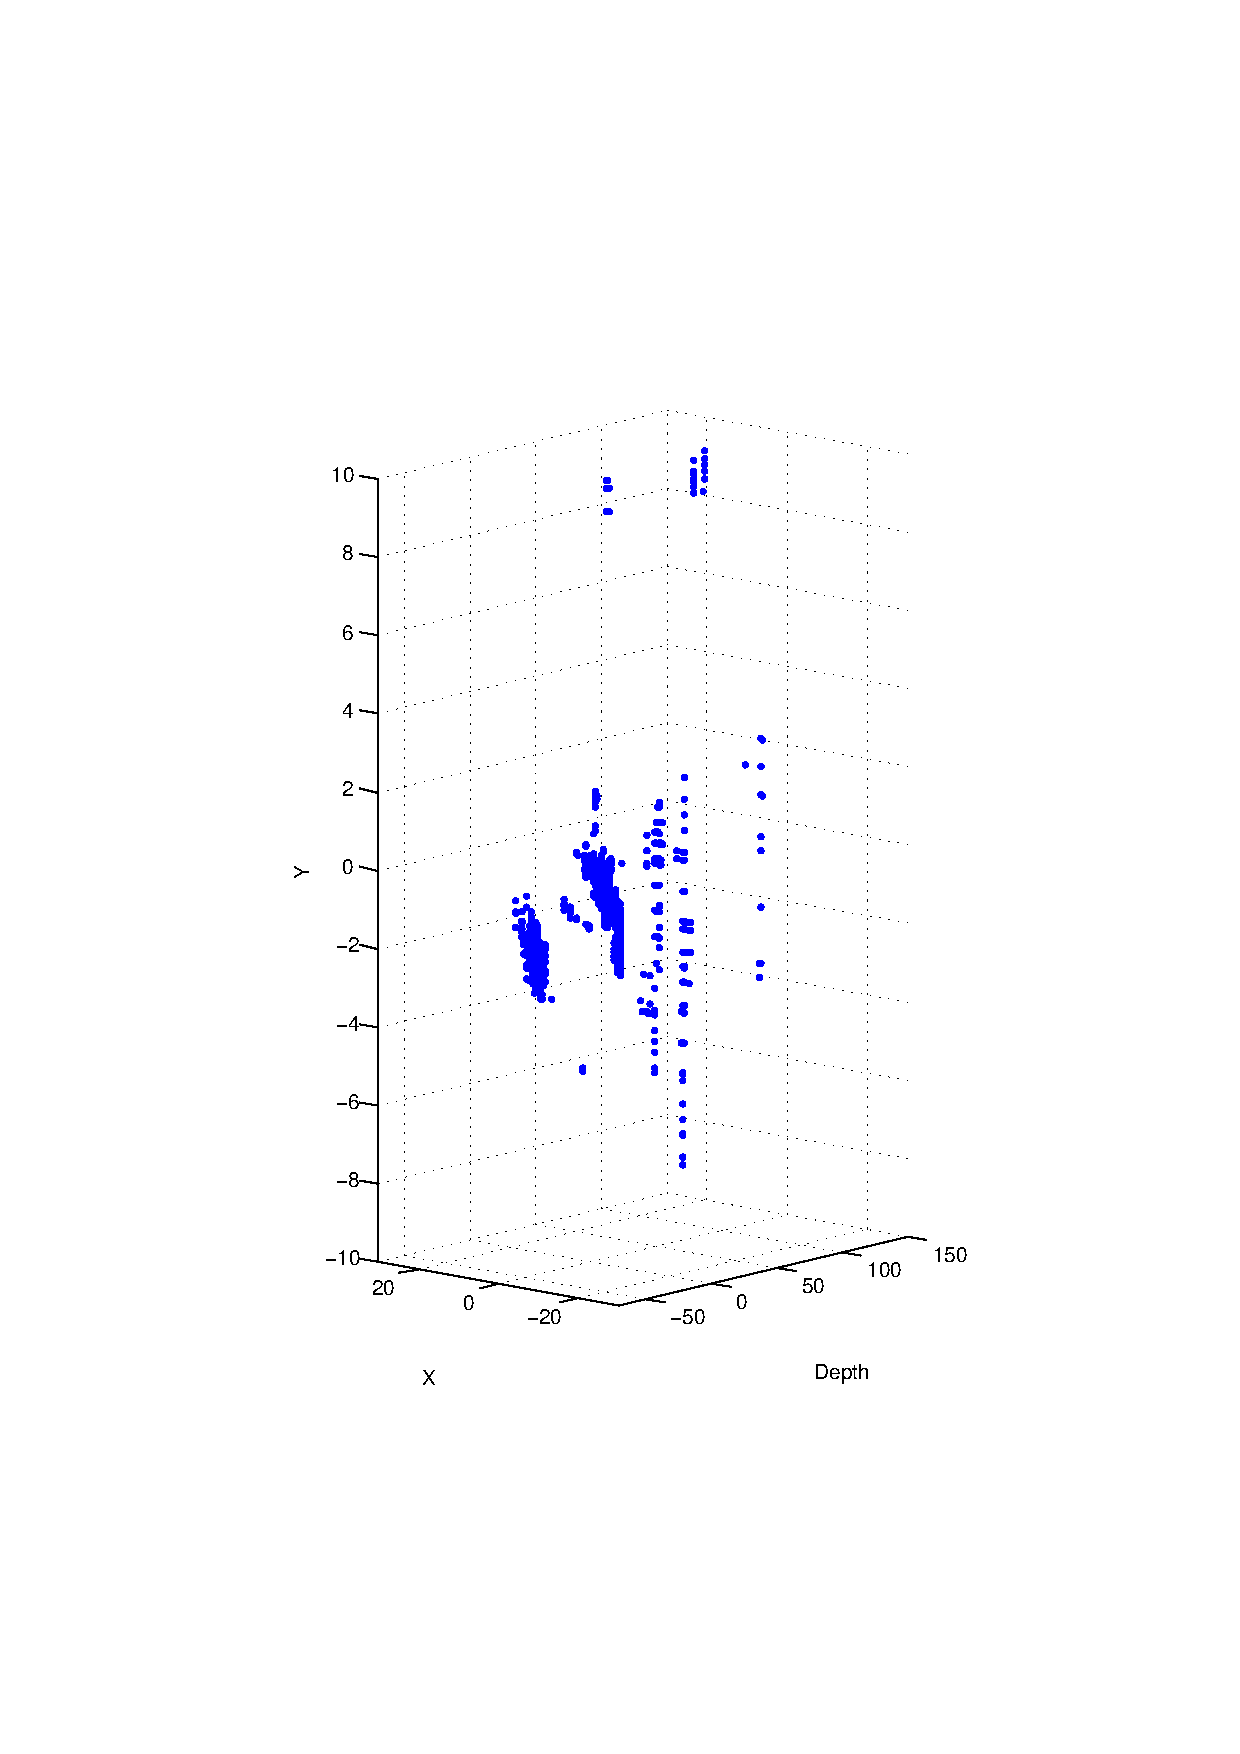
\includegraphics[width=0.6\textwidth]{pics/pos2-irregular-3d}
    \caption{Depth image from the Stereo Rig with reprojected 3d coordinates from position
    2 looking at position 1}
    \label{chap7:fig-pos2-irregular-depth}
\end{figure}
\begin{figure}[htbp]
    \centering
    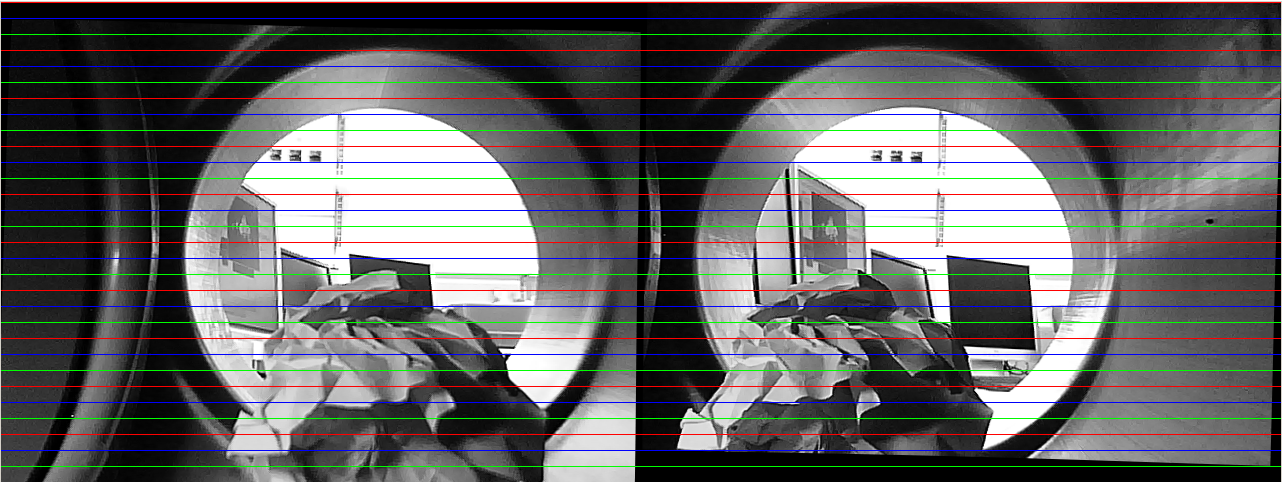
\includegraphics[width=\textwidth]{pics/pos2-irregular-rectified}
    \caption{The rectified stereo pair from position 2 looking at position 1 }
    \label{chap7:fig-pos2-irregular-rectified}
\end{figure}



\subsection{Irregular Obstacle at Point B at Position One}
This test shows how an irregular object affects the algorithms. See Figures 
\ref{chap7:fig-pos1-irregular-tof-3d}--\ref{chap7:fig-pos1-irregular-urg-2d} 
\begin{figure}[htbp]
    \centering
    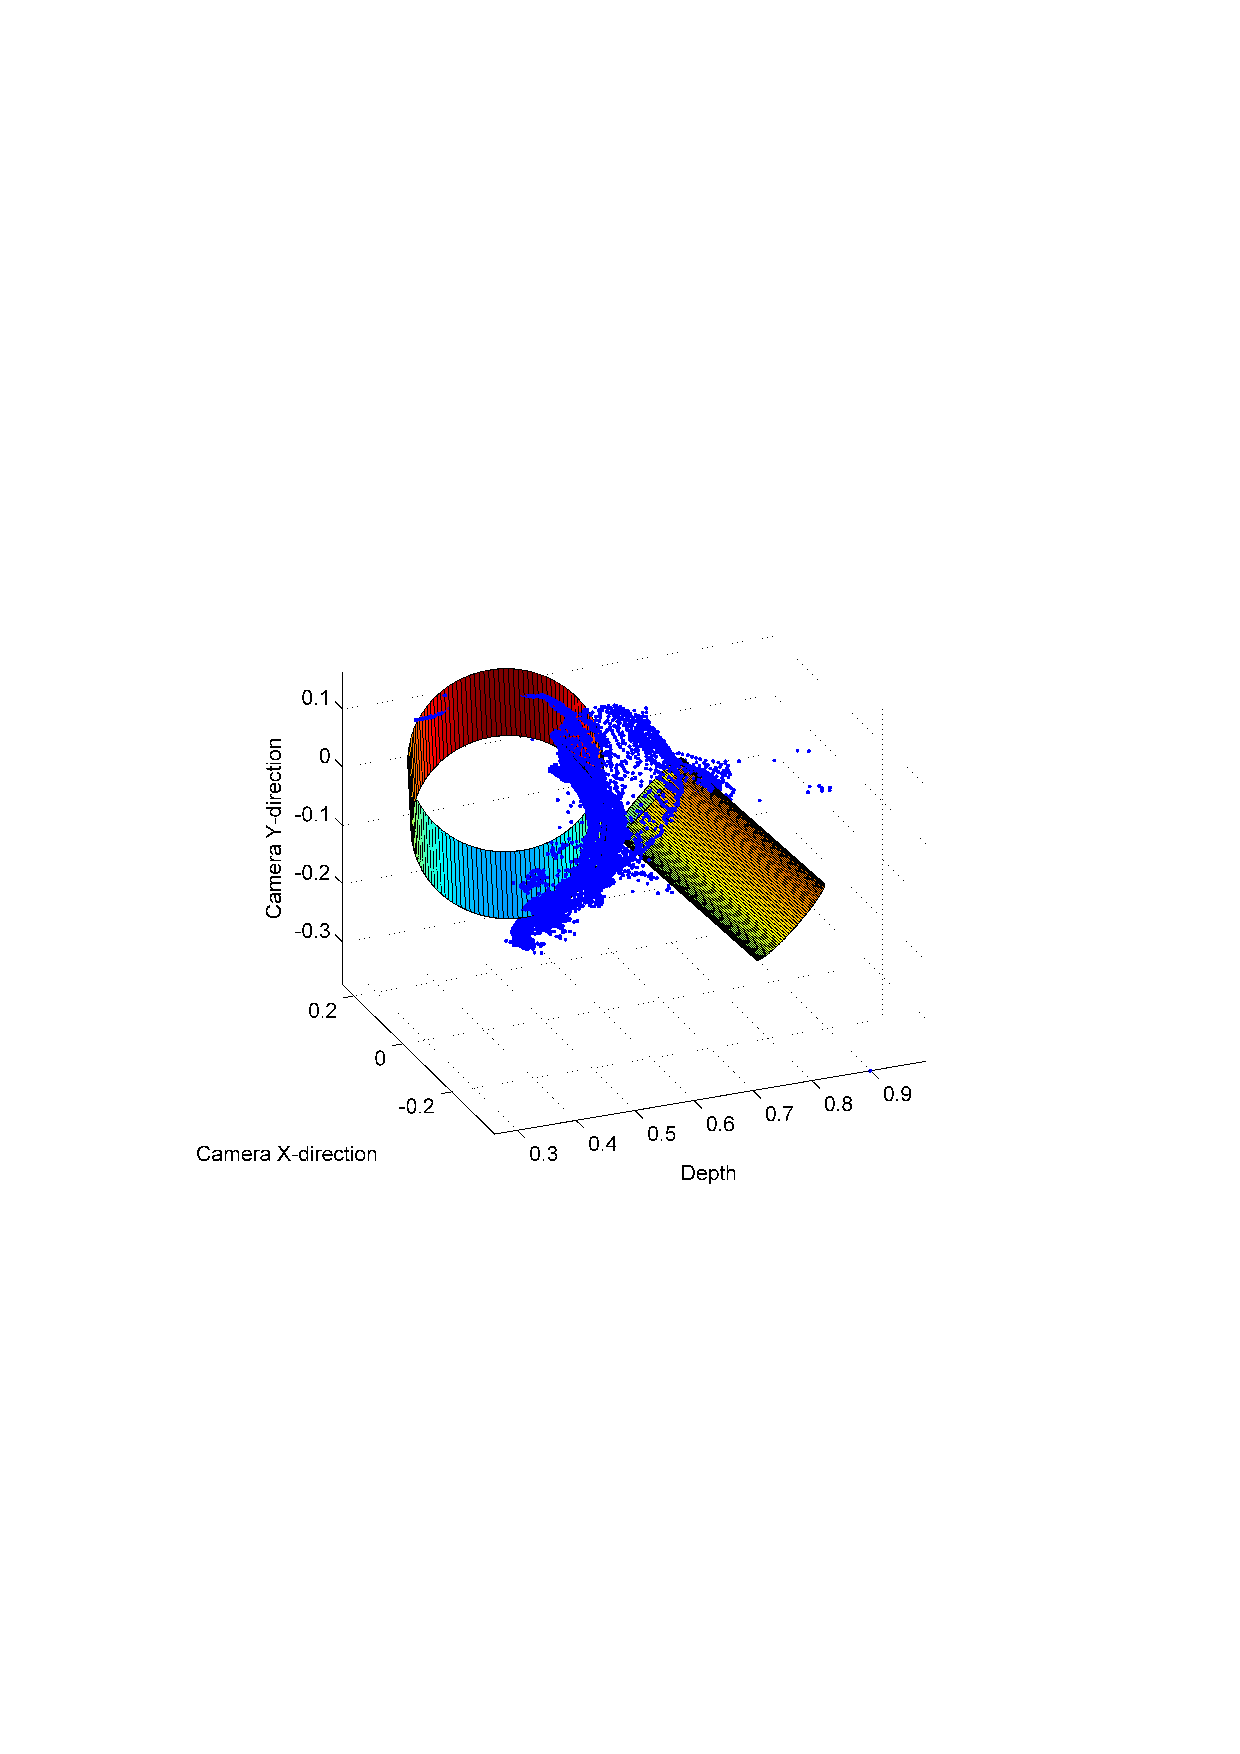
\includegraphics[width=0.8\textwidth]{pics/pos1-irregular-tof-3d}
    \caption{Fitted cylinders from ToF camera at position 1 with irregular obstacle at
    position 1}
    \label{chap7:fig-pos1-irregular-tof-3d}
\end{figure}
\begin{figure}[htbp]
    \centering
    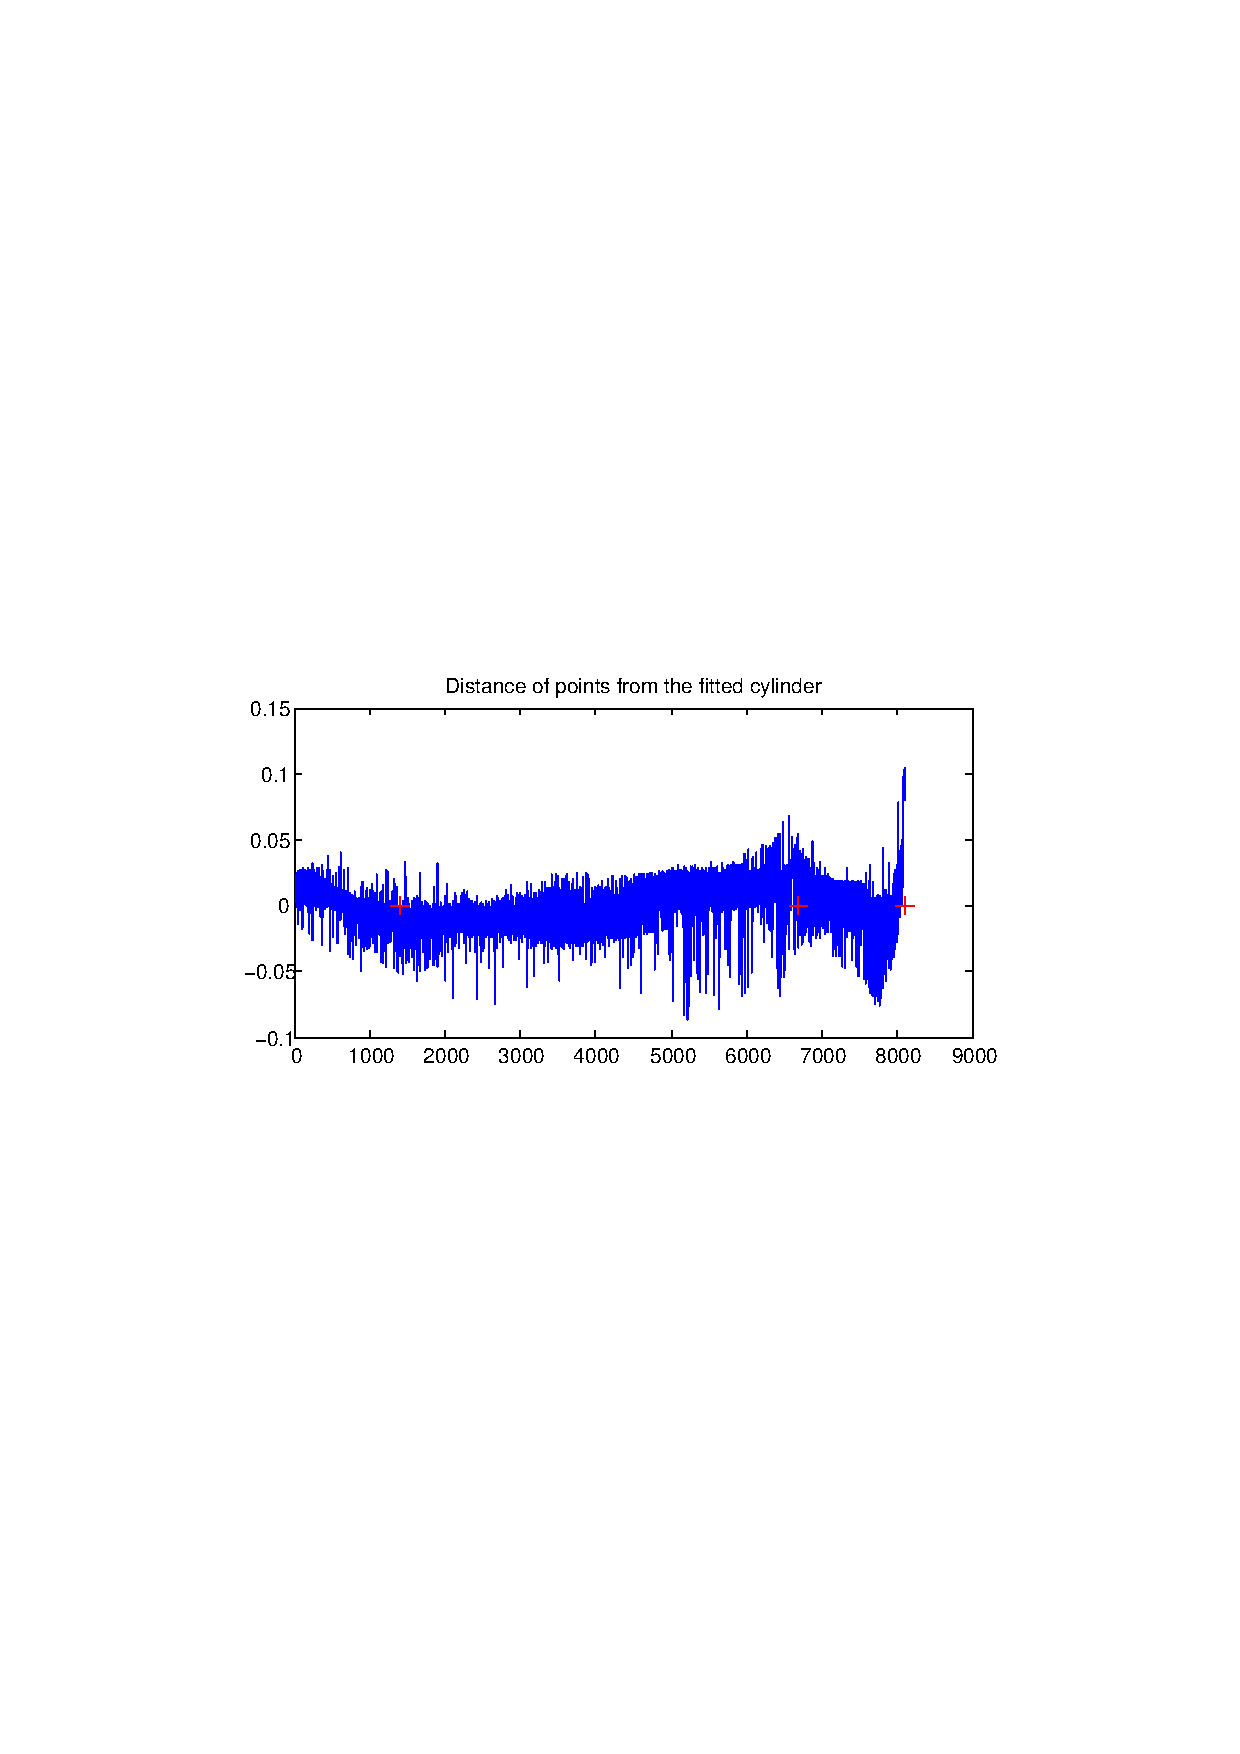
\includegraphics[width=0.8\textwidth]{pics/pos1-irregular-tof-dist}
    \caption{The distance from the fitted cylinder with irregular obstacle at position 1}
    \label{chap7:fig-pos1-irregular-tof-dits}
\end{figure}
\begin{figure}[htbp]
    \centering
    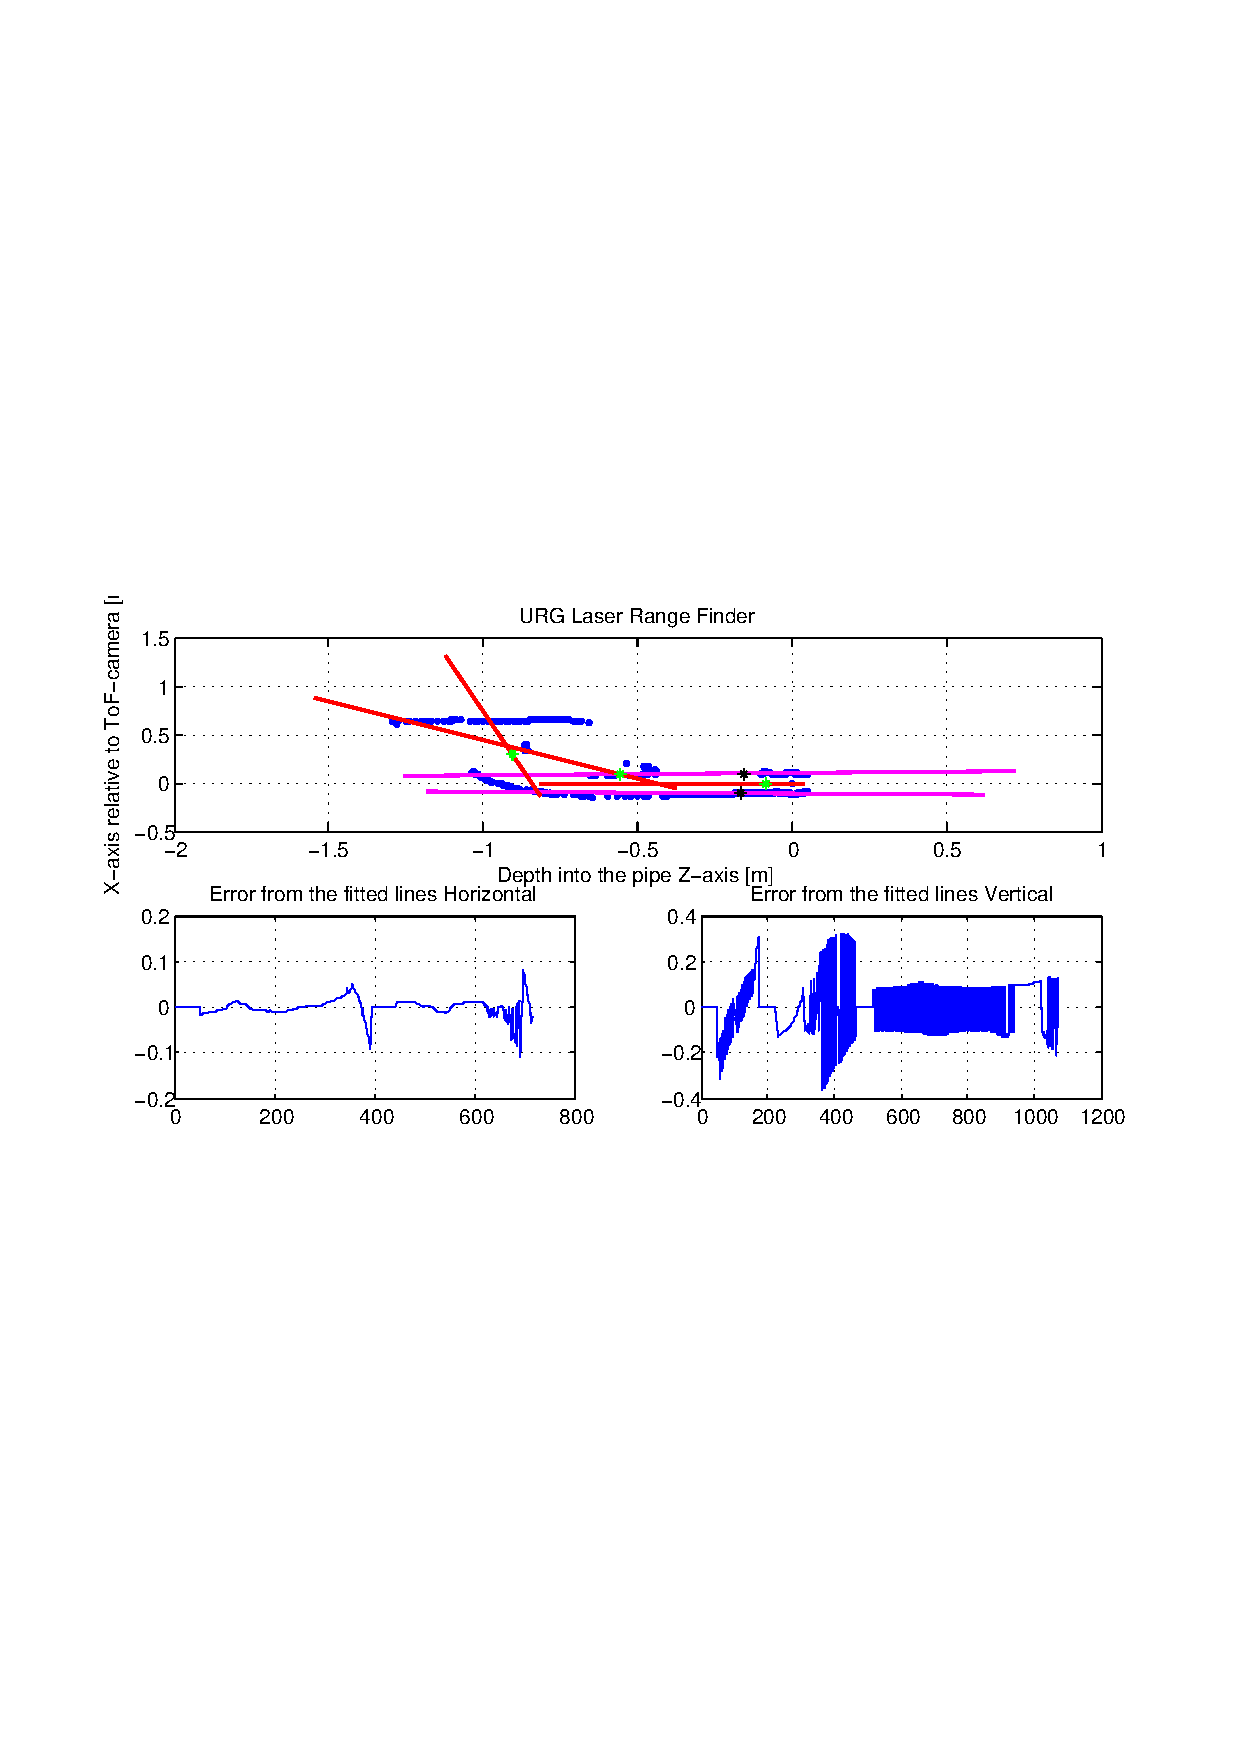
\includegraphics[width=0.8\textwidth]{pics/pos1-irregular-urg-2d}
    \caption{The data from the URG Laser Range Finder at Position 1}
    \label{chap7:fig-pos1-irregular-urg-2d}
\end{figure}
In Figure \ref{chap7:fig-pos1-irregular-urg-2d} the irregular obstacle is not showing up
on the URG. This is because the laser range finders scanner beams scans over the obstacle
and therefor does not detect it. 


\subsection{Regular Obstacle at Point B at Position One}
Figures \ref{chap7:fig-pos1-regular-tof-3d}--\ref{chap7:fig-pos1-regular-urg-2d} shows the
results from the regular obstacle test. Figure \ref{chap7:fig-pos1-regular-urg-2d} differs
from Figure \ref{chap7:fig-pos1-irregular-urg-2d} in the only way that the irregular
obstacle is not in the field-of-view of the Laser Range Finder, but the regular obstacle
is. Although, this does not seem to impact the line fit notably. 
\begin{figure}[htbp]
    \centering
    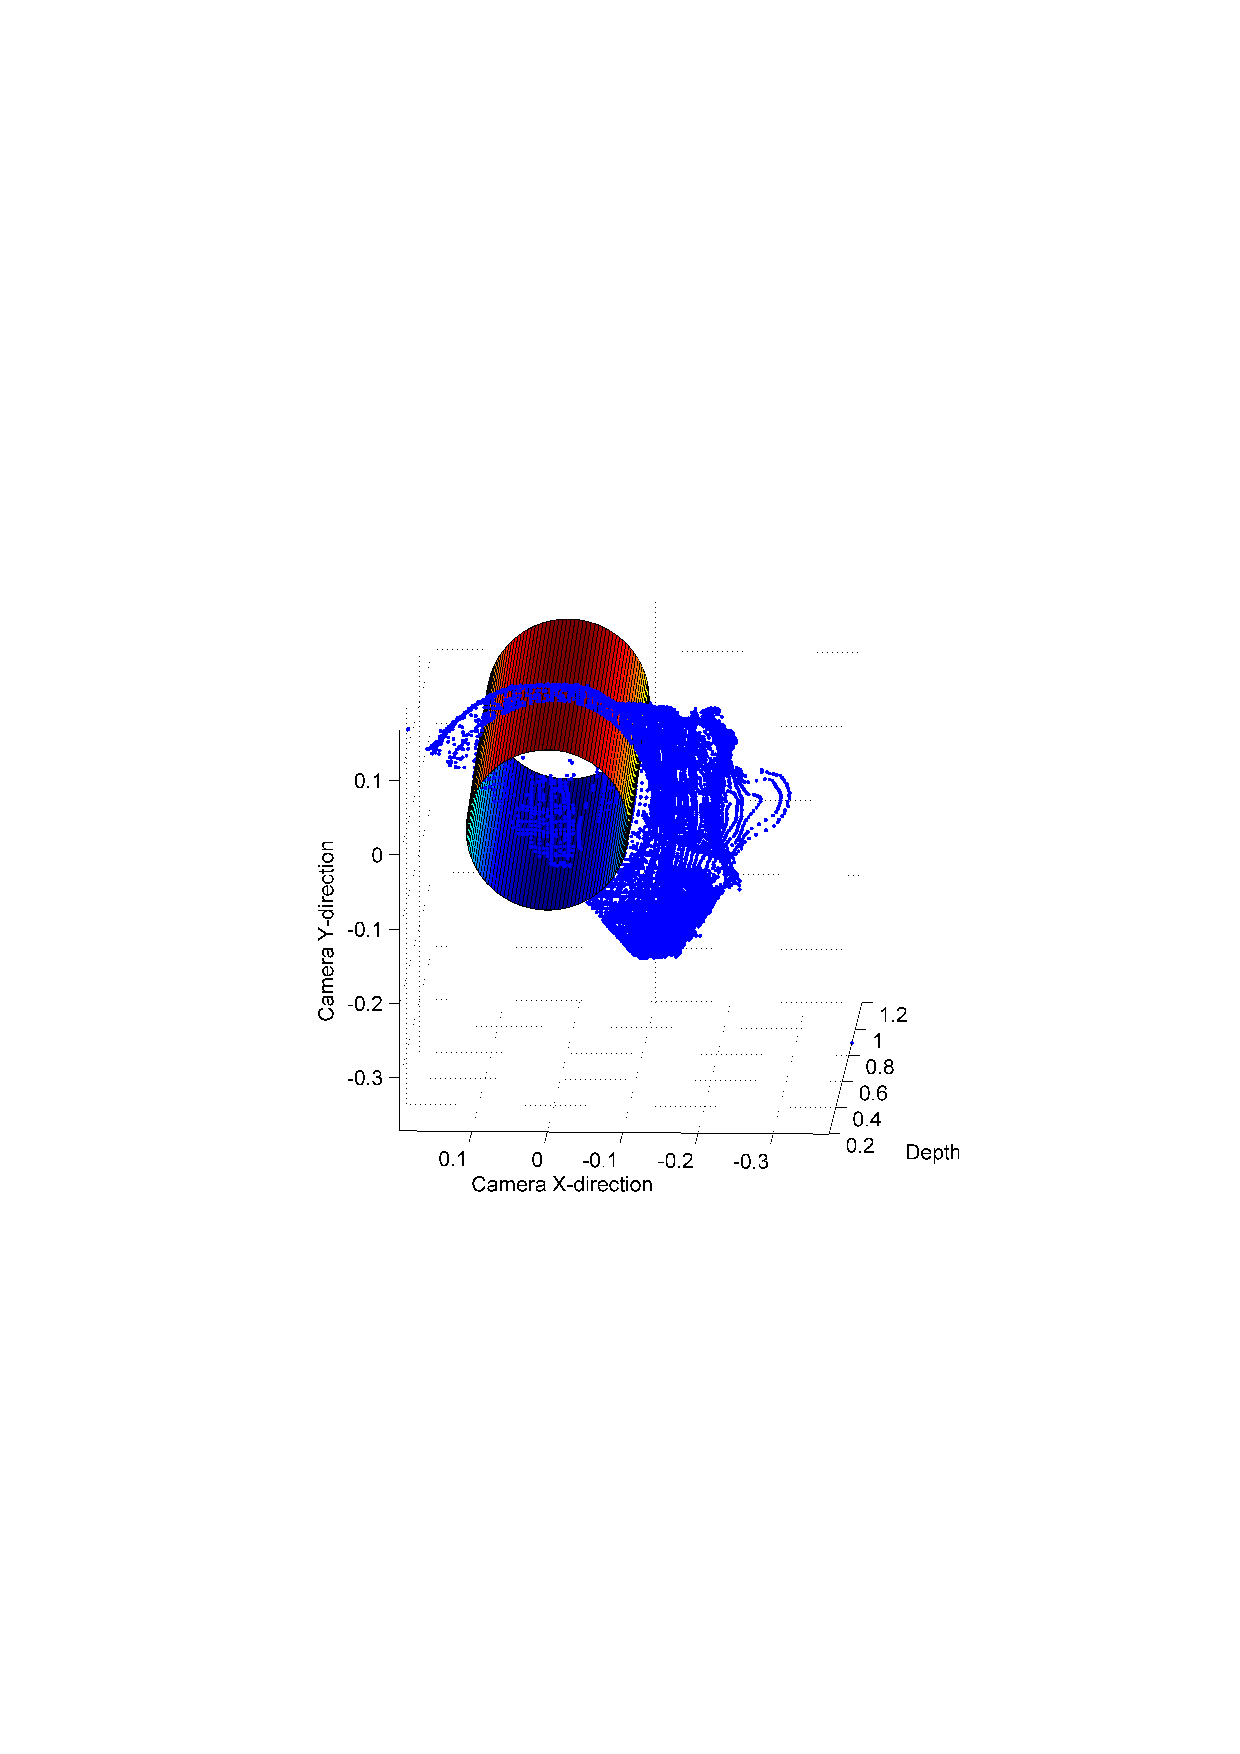
\includegraphics[width=0.7\textwidth]{pics/pos1-regular-urg-3d}
    \caption{Cylinder fitted only using the Laser Range Finder measurements at position 1}
    \label{chap7:fig-pos1-regular-urg-3d}
\end{figure}
The bottle can be seen in the middle of the fitted cylinder, represented as the point
cloud directly in the center of the cylinder. It is worth noting that the estimated
cylinder radius is smaller than the coordinates given by the time-of-flight camera. This
might be due to the fact that the height of the laser range finder in the pipe, is not
exactly known, or that the ToF-camera over-estimates the distances. 

\begin{figure}[htbp]
    \centering
    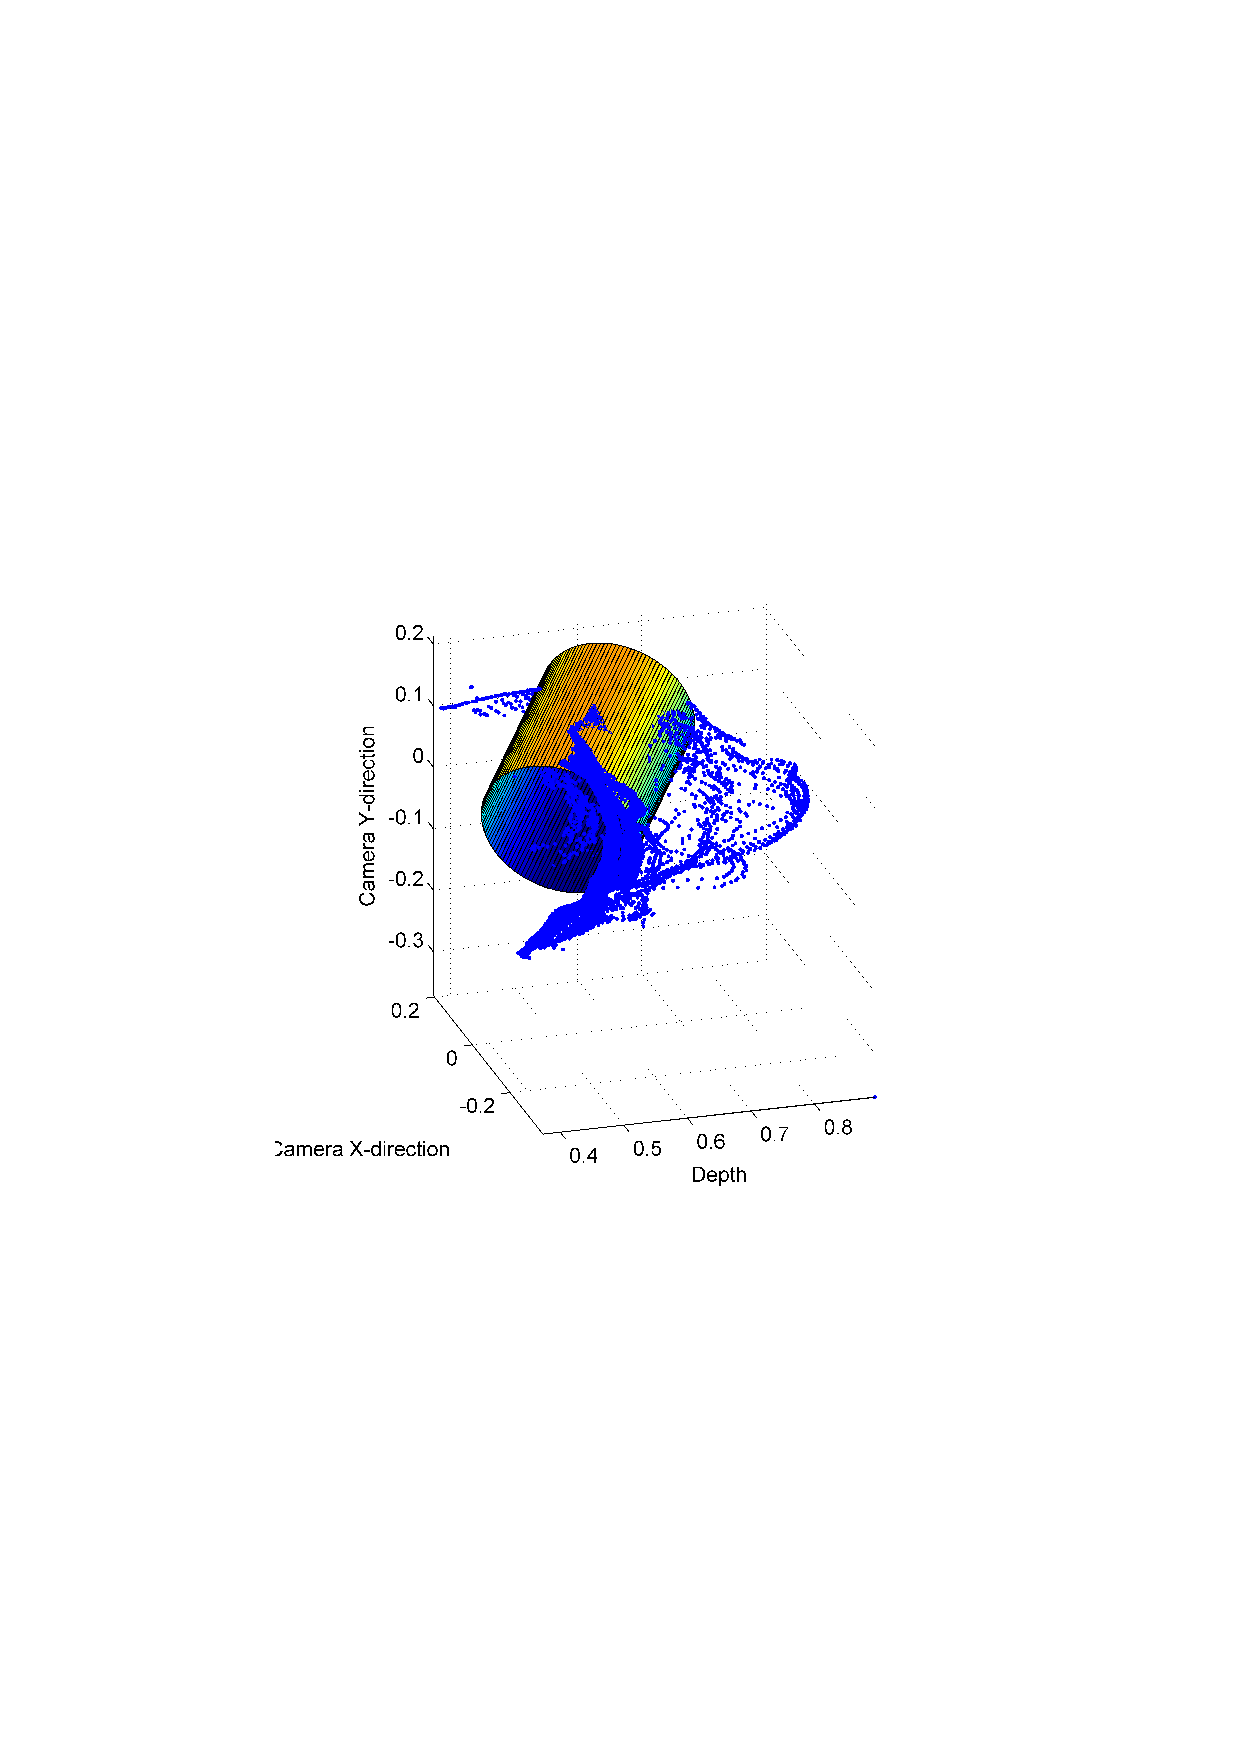
\includegraphics[width=0.7\textwidth]{pics/pos1-regular-tof-3d}
    \caption{Fitted cylinders from ToF camera at position 1 with regular obstacle at
    position 1}
    \label{chap7:fig-pos1-regular-tof-3d}
\end{figure}
\begin{figure}[htbp]
    \centering
    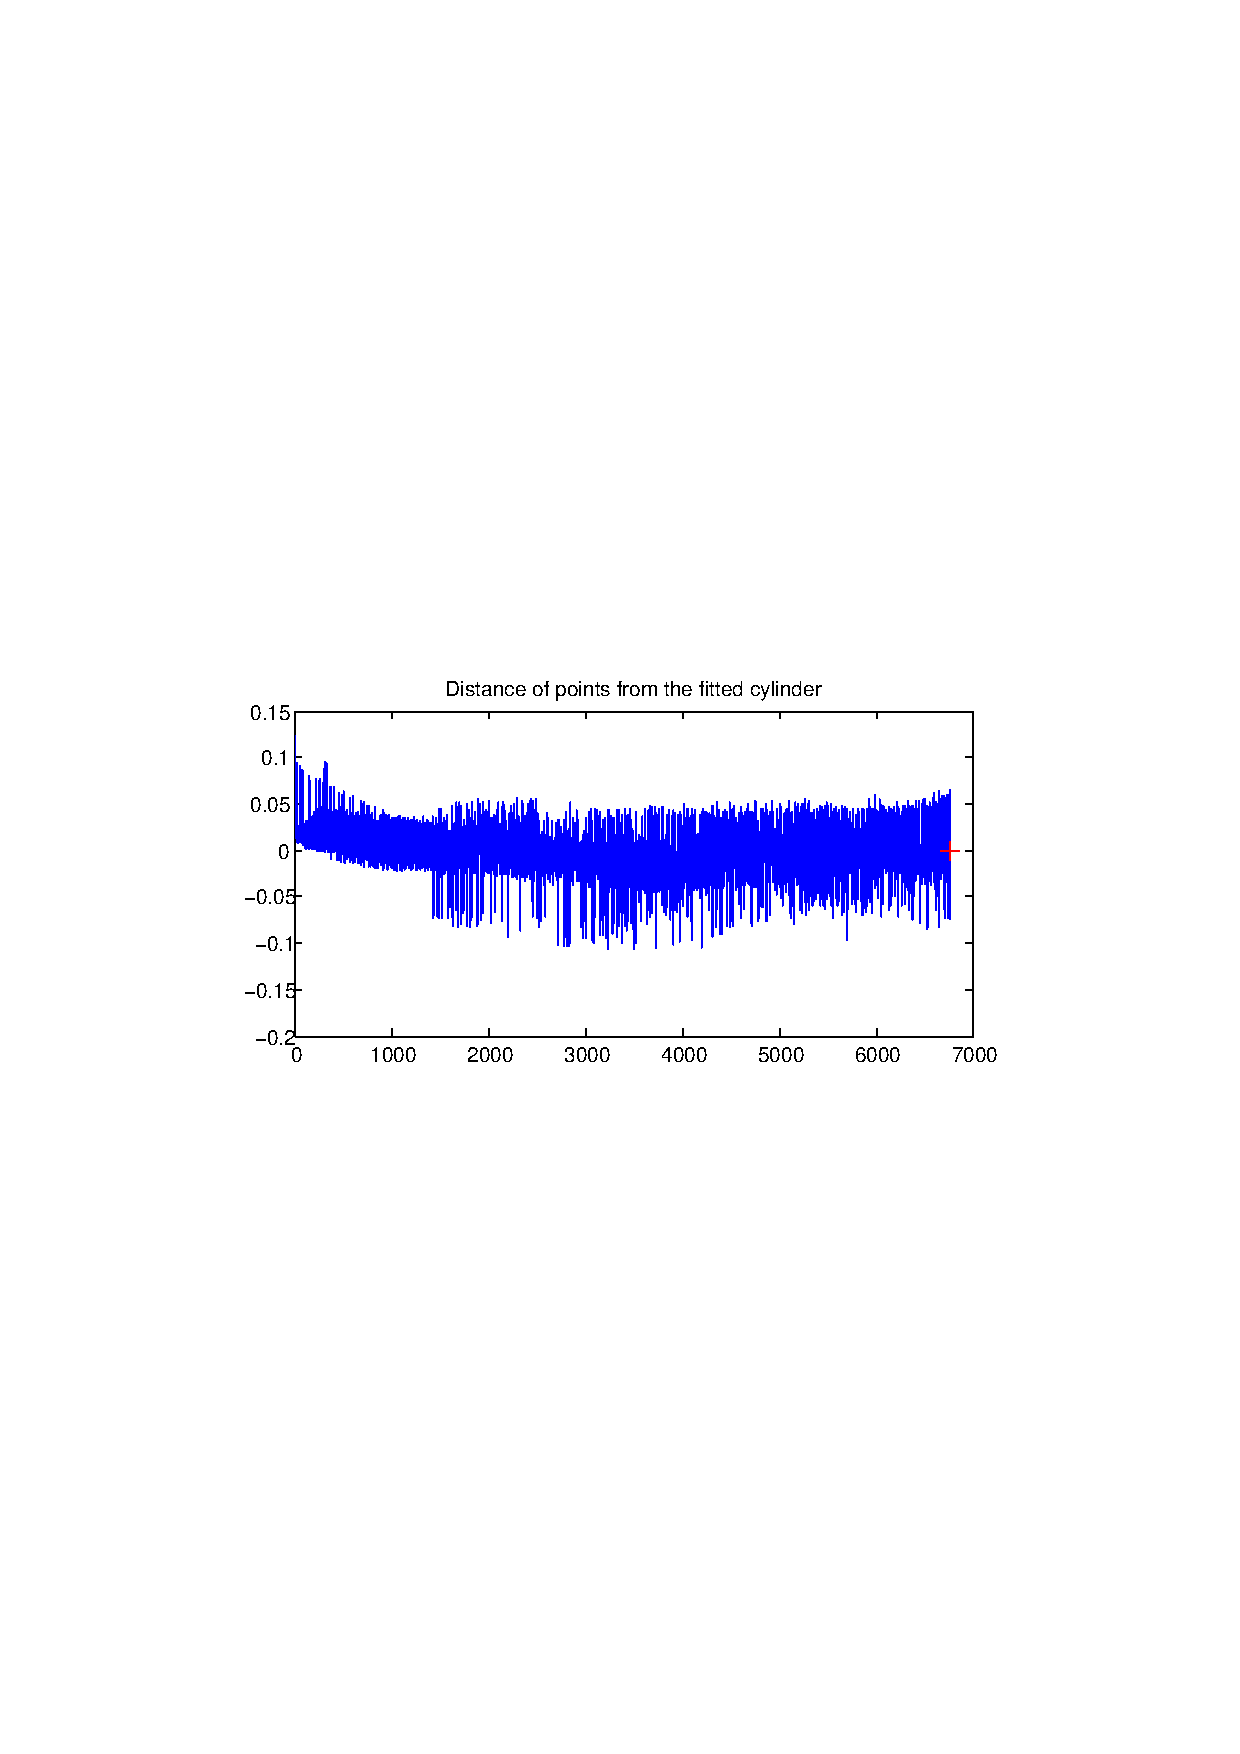
\includegraphics[width=0.8\textwidth]{pics/pos1-regular-tof-dist}
    \caption{The distance from the fitted cylinder with regular obstacle at position 1}
    \label{chap7:fig-pos1-regular-tof-dits}
\end{figure}
\begin{figure}[htbp]
    \centering
    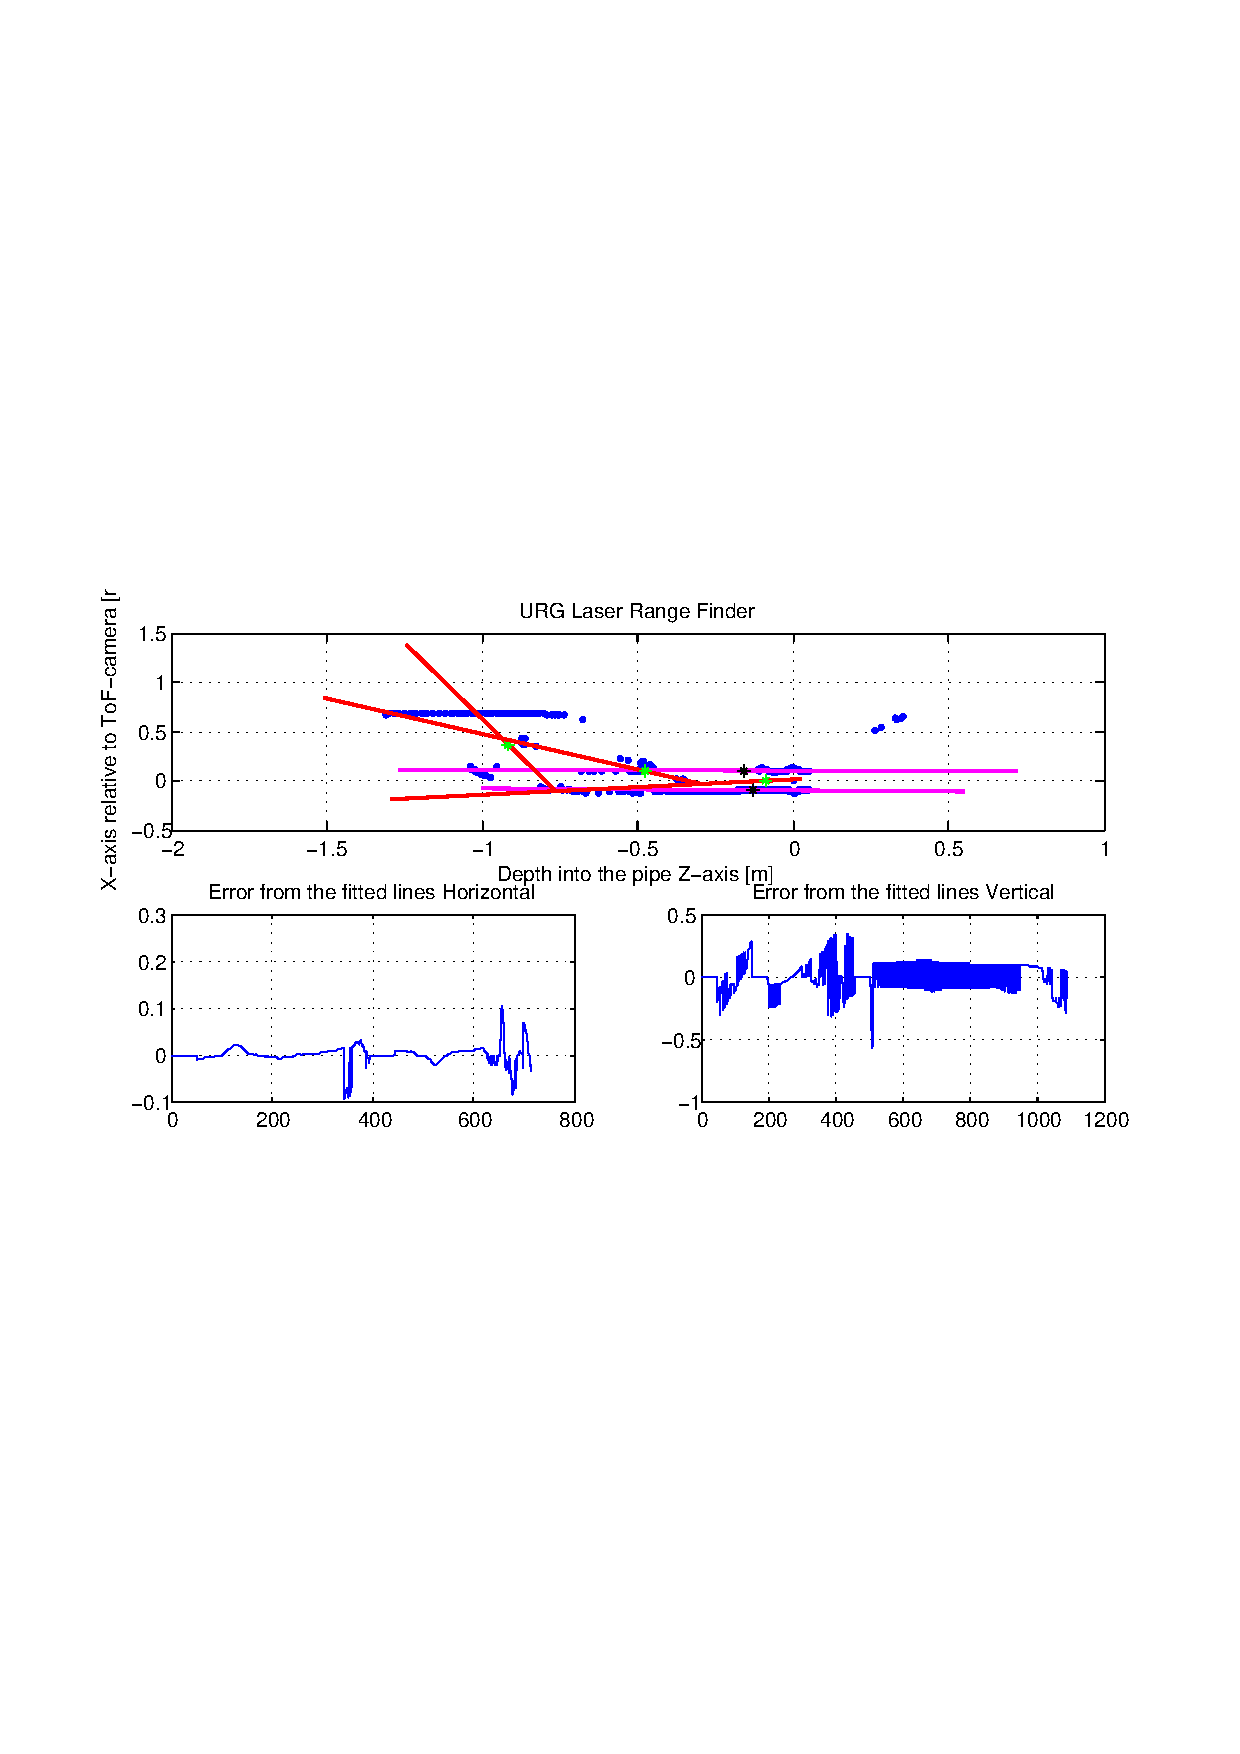
\includegraphics[width=0.95\textwidth]{pics/pos1-regular-urg-2d}
    \caption{The data from the URG Laser Range Finder at Position 1}
    \label{chap7:fig-pos1-regular-urg-2d}
\end{figure}
\begin{figure}[htbp]
    \centering
    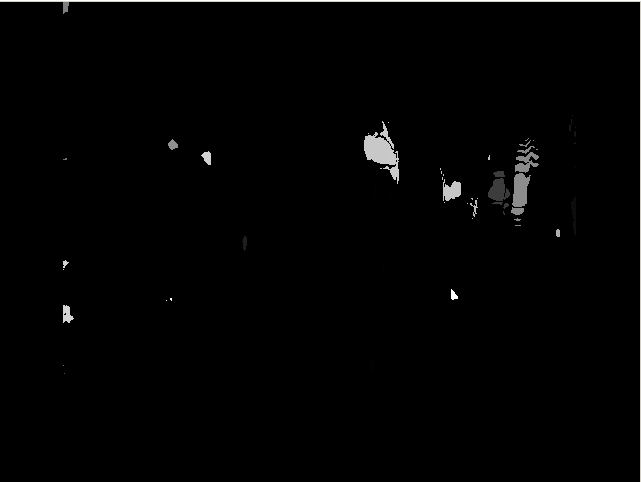
\includegraphics[width=0.5\textwidth]{pics/pos1-regular-depth}
    \caption{Disparity and depth image of regular obstacle at Position 1}
    \label{chap7:fig-pos1-regular-depth}
\end{figure}
\begin{figure}[htbp]
    \centering
    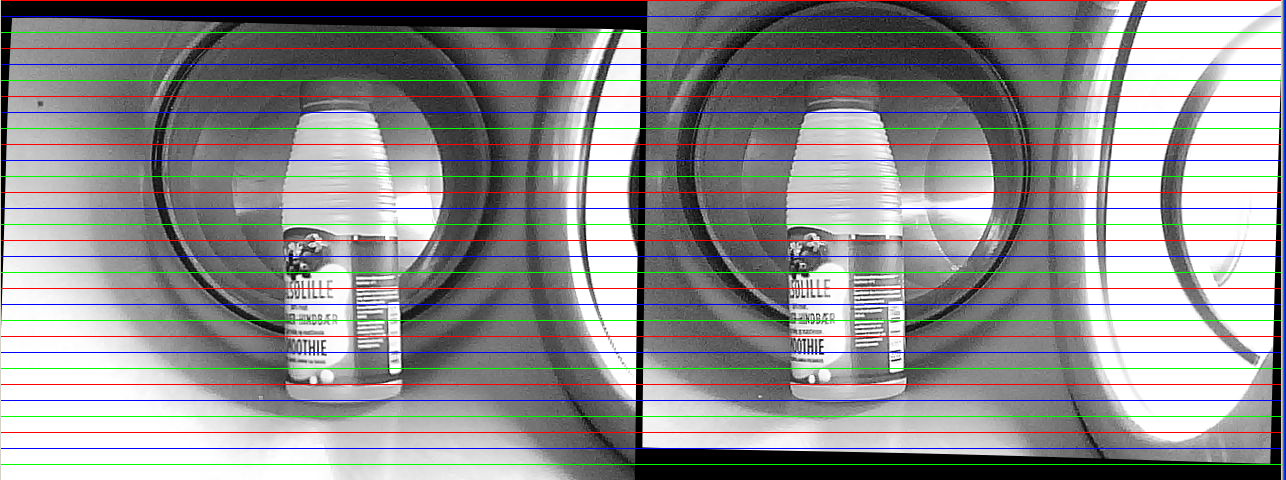
\includegraphics[width=\textwidth]{pics/pos1-regular-rectified}
    \caption{Rectified images of regular obstacle at Position 1}
    \label{chap7:fig-pos1-regular-rectified}
\end{figure}

